
\documentclass[12pt,a4paper]{article}
%

\usepackage{pa}      % by Jonathan Katz

% hyperlinks and metadata
\usepackage[bookmarks, breaklinks, pdftitle={neta}, pdfauthor={François Briatte}]{hyperref}

% TABLES AND FIGURES
\usepackage{caption} % boring margin work
\usepackage{subcaption}
\newcommand{\legend}[1]{\vspace{1em}\caption{#1}}
\newcommand{\sublegend}[1]{\subcaption{#1}\vspace{1em}}
\usepackage{multicol} % bibliography

% ---- PAGES
\usepackage{geometry} 
\geometry{a4paper, textwidth=5.5in, textheight=9.6in, marginparwidth=.6in}
\setlength\parindent{0em}
\setlength{\parskip}{1em}
\usepackage{setspace}
\doublespacing

% \usepackage[style=chicago-notes,url=false,doi=false,isbn=false,maxnames=2,maxbibnames=2,firstinits,sorting=none,backend=biber]{biblatex}
% \bibliography{neta.bib}
\usepackage{natbib}
\renewcommand{\harvardurl}{URL: \url}

% ---- FONTS
\usepackage[utf8]{inputenx}
\usepackage[english]{babel}

% \usepackage[greek=n]{libgreek}
\usepackage{libertine}
\usepackage[scaled=.92]{inconsolata} % not working with '$' or '<-' etc.
% \usepackage[defaultmathsizes]{mathastext}
% \usepackage{microtype}

% ----- MATH
\usepackage{amsmath}
\usepackage{amssymb}
\usepackage{bm}
\newcommand\vm[1]{% by Donald Arsenau
\bm{\mathrm{#1}}}

\usepackage{endnotes}



\title{\large Network Patterns of Party Polarization \\ in the French Parliament}
\author{\href{mailto:f.briatte@ed.ac.uk}{François Briatte}}
\date{\today}

\begin{document}

	\maketitle
  \begin{abstract}

    % 96 words
    This paper measures the extent of party polarization in the French Parliament politics through the ebb and flow of legislative collaboration between its members. Drawing extensively on existing studies of cosponsorship networks in the U.S. Congress, we introduce similar data for both legislative chambers over the past seven legislatures. We then use exponential graph models to measure the influence of party affiliation on the likelihood of cosponsorship since 1986. Like roll-call spatial voting models of French legislative politics, our results tend to reveal a primarily one-dimensional policy space structured by left-right politics and strong party loyalty.%
      % 30 words
      \endnote{The author thanks Baptiste Coulmont for inspiring this study, Martial Foucault for helpful suggestions, Jonathan Chibois and Sébastien Dubourg for discussing Senate data availability, and Mason Porter for replication material.}%

\end{abstract}



  %\tableofcontents
  %\newpage

  \clearpage
  \section{Introduction}\label{sec:intro}%
  % intro

Previous studies of (co)sponsored legislation have found it to be a useful heuristic to how Members of Parliament (MPs) signal positions to other legislators \citep{KesslerKrehbiel1996-APSR}, to the executive, or to constituencies such as interest groups and voters \citep{WilsonYoung1997-LSQ}. This kind of position taking is further encouraged by the weakly constrained nature of (co)sponsorship, over which legislators generally enjoy more control than they do over votes \citep{Schiller1995-AJPS}.%

A large fraction of existing research on legislative networks is based on U.S. legislative chambers, for which there are large scale historical data available \citep{ZhangFriend2008-P,ClarkOsborn2009-SPPQ}. Drawing extensively from this literature, this paper examines the extent of party polarization expressed by members of the French Parliament through their propensity to cosponsor legislation together, as an alternative  measurement strategy to roll-call voting records \citep{Sauger2010}.%

Section~\ref{sec:data} starts by introducing original network data built from around 100,000 cosponsored amendments and bills introduced in both chambers of the French Parliament over the past 27 years. Section~\ref{sec:methods} then presents a methodological framework that relies on exponential random graph models \citep{KrivitskyHandcock2009-SN,CranmerDesmarais2011-PA} to measure the influence of party identification on cosponsorship in each of the seven parliamentary legislatures since 1986.%

In accordance with roll-call spatial voting models of French legislative politics \citep{GodboutFoucault2013-FP}, the results presented in Section~\ref{sec:results} tend to reveal a primarily one-dimensional policy space structured by left-right positions and strong party loyalty. Both random and fixed effects models of the cosponsorship data find moderate to strong party-based network patterns across all parliamentary groups that are largely consistent with longer historical patterns of party unity in postwar France \citep{Sauger2010}.%

The overall results of our study, which we further discuss in Section~\ref{sec:discussion}, show that party polarization has increased in recent legislatures, as Members of Parliament sponsor more and more legislation within party lines. The two-by-two multi-party configuration popularized decades ago by \citet{Duverger1968-PUF} under the name ``quadrille bipolaire'' is still empirically relevant to qualify both past and present left-right coalitions in Parliament, and is highly predictive of legislative interactions conducted under the control of highly disciplined party coalitions.%


  \section{Data}\label{sec:data}%
  % data

Although formally intended to encourage technical collaboration between branches of government over lawmaking \citep{Heller2001-AJPS}, legislation also translates the struggle of government branches over the control of the legislative agenda. In several studies of U.S. legislatures, this struggle has been shown to form regular patterns of collaboration between legislators, the structure of which can help predict legislative productivity \citep{Fowler2006-PA,ChoFowler2010-JP}.%

Members of the French Parliament are provided limited resources and enjoy only restricted control over the legislative agenda in comparison to the executive \citep{Kerrouche2006-JLS,BaumgartnerBrouard2014-G}. In that context, many bills introduced by MPs represent attempts by opposition parties to express defiance at the government and obstruct its legislative drive \citep{Conley2011-FP}. Similarly, a large volume of amendments produced during parliamentary plenary debates serve to grant their authors a few minutes of speaking time during the passage of a bill.%

Legislation therefore plays a role in framing parliamentarians as veto players in the policy process \citep{Tsebelis1999-APSR}. For that reason, as a previous study of the French National Assembly has observed, ``the volume of private members' bills, especially those from minority deputies, may be regarded as a reasonable proxy for the level of conflict between the government and opposition deputies. It will also reveal something of the extent of the government’s political control over its backbenchers'' \citep[p.~343]{Kerrouche2006-JLS}.%

\subsection{Sample definition}

In this study, we focus on the relational determinants of legislative behaviour, and measure legislative collaboration with the aim to control, rather than to account, for the volume of legislation passed. Our sampling frame thus consisted in all available legislation for which one MP could be nominally identified as the author, and one or more other MP(s) could be nominally identified as cosponsor(s). This design concentrates on ties between first authors and their cosponsors within each chamber, as does \citet{Fowler2006-PA} on similar data.%

The legislation collected for this research consist of slightly over 103,000 items sponsored over the past 27 years, from 1986 to today. The 96,168 amendments and 6,864 bills used to build the cosponsorship networks presented in the next sections are distributed over seven legislatures, or roughly half of the Fifth Republic, and come from a larger sample approximately twice that size, which also includes single-sponsored MP legislation, government bills and nonbinding resolutions.%

The data were produced by scraping sponsor details from the National Assembly (\url{http://www.assemblee-nationale.fr/}) and Senate (\url{http://www.senat.fr/}) websites. Legislation data for the National Assembly were retrieved from its online pages, and legislation data for the Senate were retrieved from the SQL database dumps of its open data initiative (\url{http://data.senat.fr/}). Less than 2\% of the data could not be processed due to missing information or parsing issues.%

Figures~\ref{fig:counts_an} and~\ref{fig:counts_se} show the time distribution of the data over each National Assembly term (\emph{législature}), which coincide with executive terms from 2002 onwards. Legislatures~8 (1986-1988), 10 (1993-1997) and 11 (1997-2002) include periods of divided government \citep{BaumgartnerBrouard2014-G}, with three leftwing parties in government during legislature~11; all other periods represent periods of government under leftwing or rightwing two-party coalitions.%
  % \endnote{See \citet[p.~313]{GodboutFoucault2013-FP} for more exhaustive information on parliamentary legislatures in the Fourth and Fifth Republics. The data collected for this study contain only basic MP socio-demographics; for a more detailed examination, see \citet{FrancoisGrossman2011-I}.}%

$$\textrm{[FIGURE~\ref{fig:counts}]}$$

Table~\ref{tbl:counts} provides further information on the number of MPs and parliamentary party groups represented in the cosponsorship data. The number of MPs per legislature is sometimes superior to the number of seats due to replacements and delays in legislation that allowed sponsors from multiple legislatures to cosponsor the same bill. The number of groups indicates how many parties have more than 9 members in the cosponsorship sample, which is the lowest threshold to form a party group in (Senate) parliamentary rules.%
  %
  \endnote{The threshold to form a party group in the National Assembly was lowered from 20 to 15 members in 2009. Our figure futher ignores unaffiliated MPs.}%

$$\textrm{[TABLE~\ref{tbl:counts}]}$$

The most serious limitation in the data explains the highly unequal number of items before and after 2002  in both chambers: amendments data were available only since 2004 in the National Assembly or since 2001 in the Senate, and do not include amendments submitted to specialised committees, where a lot of ``invisible'' legislative collaboration occurs \citep[p.~357]{Kerrouche2006-JLS}. Another major issue specifically affects legislature~10 in the National Assembly bills series, which is composed of only a few cosponsored bills at the end of the legislature. For both reasons, we first ran our analysis on amendments and bills separately, and then on the combined series.%

\subsection{Network construction}

Cosponsorship networks were built out of the ties formed between the first author of a bill amendment, and all other sponsors of the proposed legislation. This definition of network ties matches the criteria used in network analyses of cosponsorship in the U.S.~Congress \citep{Fowler2006-PA,GrossShalizi2012}, and relies on a similar constructor, namely a two-mode edge list of the form%

 \[ \begin{array}{cccccc}
    	\{ a_8 , b_1 \} , & \{ a_{31}, b_1 \} , & \{ a_{27}, b_2 \} , & \dots & & \\
    	\vdots & & & & & \\
      & & & \dots & \{ a_{36}, b_{n-1} \} , & \{ a_{120}, b_n \}
    \end{array} \]

with MP sponsors denoted $a_i$ and legislation items denoted $b_k$, regardless of their kind. The construct under examination is therefore an initially bipartite, or two-mode, network of $a \times b$ ties between MPs and legislation items. To focus the study on collaboration between legislators, we collapse this construct to a one-mode network containing strictly MPs, by connecting the first author of each item to all other sponsors of the item. The resulting adjacency matrix $A$ of directed ties between MPs $(i,j)$ is an asymmetric matrix with elements%

    \[ A(i,j) = \left\{
      \begin{array}{l l}
        1 & \quad \text{if MP $j$ cosponsored an amendment or bill by MP $i$,}\\
        0 & \quad \text{otherwise.}
      \end{array} \right. \]

and where all diagonal elements describing network self-loops --- MPs hypothetically cosponsoring legislation with themselves --- are discarded.%

%  The network can be described as a directed edge list of the form%
%
%  \[ \begin{array}{cccccc}
%       \{ i_8 , j_{15} \} , & \{ i_{8}, j_{190} \} , & \{ i_{31}, j_2 \} , & \dots & & \\
%       \vdots & & & & & \\
%       & & & \dots & \{ i_{120}, j_{43} \} , & \{ i_{120}, j_{48} \}
%     \end{array} \]

Since cosponsorship between MPs $i$ and $j$ can occur more than once during a legislature, the ties of their network must then be valued to reflect their different strength. To do so, we followed \citet[Equation.~1]{GrossShalizi2012} by weighting all cosponsorships in inverse proportion to the overall number of cosponsors on the item, and by normalizing their sum to the maximum number of possible cosponsorships between MPs $i$ and $j$.%
  %
  \endnote{The resulting weights are bounded between $0$ and $1$ and are approximately log-normal in several of the collected networks.}%

Finally, for the purpose of this study, we recoded a myriad of parliamentary party group affiliations to a simplified list of seven leftwing and rightwing political families. Our recoding is broadly similar to that of \citet[p.~310]{GodboutFoucault2013-FP}: for instance, we also coded the Red-Green leftwing `GDR' coalition of legislature~13 (2007-2012) as a single group. This classification offers a spectrum of four leftwing and three rightwing party groups: Communists/Red-Greens, Greens, Socialists and Radicals on the leftwing, and Centrists, Conservatives and the \emph{Front national} on the rightwing.%
  %
  \endnote{The \emph{Front national} formed a single party group in legislature~8 of the National Assembly (1986-1988).}%

Three slight differences exist between our classification and the one used by \citet[p.~310]{GodboutFoucault2013-FP}. First, in order to better capture leftwing party divisions (especially in the Senate), we did not collapse Radical MPs with Socialists MPs when both formed separate parliamentary groups. We also decided to code \emph{Démocratie libérale} (DL) National Assembly MPs as rightwing Conservatives (RPR/UMP) rather than Centrists. Last, we left all unaffiliated MPs (\emph{non inscrits} and \emph{sans étiquette}) out of our classification. These differences create nontrivial differences in party codes between both classifications, but do not seriously threaten the overall comparability of the samples used.%

The replication material for this paper, which was written in \texttt{R}~\citep{R}, contains all necessary functions to download the raw data and process it to weighted network objects, which can be easily visualized using several placement algorithms \citep{Butts2008-JSS} or converted to other formats. The replication material contains the postprocessed legislation data up to April 6, 2014, which we used in the present analysis. %
   \endnote{See \url{https://github.com/briatte/neta}. The replication material can update the data past its current endpoint, so that legislature~14, which started in 2012, can be supplemented with more information as it becomes available.}%


  \section{Methods}\label{sec:methods}%
  The cosponsorship networks under study are large-scale objects built out of primarily weak signals between individual actors (MPs) who carry only limited information with regards to the overall topology of legislative collaboration occuring in the network as a whole. Assessing the extent of cohesion or divisiveness expressed at the level of parliamentary party groups therefore requires paying attention to the structural properties of cosponsorship networks along other covariates \citep{KirklandGross2012-SN}.%

For this reason, we focus our analysis on characterizing each legislature through network-level properties, rather than through ego-level measures of influence such as rankings of MPs by legislative productivity. In order to preserve some of the benefits of exploring egocentric networks \citep[see, e.g.]{Box-SteffensmeierChristenson2014-SN}, we offer an interactive visualization of the cosponsorship network data, available online at \url{http://briatte.org/sigma}, that shows force-directed graph representations of the fourteen networks under study.%

We start by measuring the overall level of party polarization in the cosponsorship network of each legislature, finding variations in time as well as between chambers that are consistent with previous studies of party cohesion in the French Parliament. We then explain how we estimated party effects through exponential random graph models, using both random and fixed effects approaches \citep{KrivitskyHandcock2009-SN,CranmerDesmarais2011-PA}.%

\subsection{Network measures}

Figure~\ref{fig:measures} shows some weighted network properties for the fourteen legislature networks present in the data. The top row of graphs shows counts of nodes and ties in each networks, with a clear difference in network density when large volumes of amendments data are available in the series. The middle row shows weighted graph-level measures of centralization, distance and clustering in the networks \citep{OpsahlPanzarasa2009-SN,OpsahlAgneessens2010-SN}, which underline the higher intensity of cosponsorship activity in the National Assembly, in which cosponsors are more connected, more clustered and more numerous overall.%

$$\textrm{[FIGURE~\ref{fig:measures}]}$$

% Several of our network measures are expected to behave as mere covariates to the amount of available network data. In recent legislatures, for example, changes in centrality indices like betweenness \citep{Brandes2001-JMS} correlate with the inclusion of amendments data, and is not expected to reflect substantive changes in parliamentary collaboration. However, in the same legislatures, higher numbers of distinct parliamentary groups also translate into more opportunities for MPs to associate with cosponsors outside of their own party, which results in higher network-level opportunities for brokerage across structural holes, and therefore lower node-level network constraint \citep{Burt2004-AJS}.%

The bottom row of network measures provides information on network modularity, which compares the proportion of network ties formed within a given vector of groups to that same proportion in a randomized network of identical dimensions. The further away the observed network is from the randomized `null' model, the more efficient the group vector is at partitioning the network into meaningful communities \citep{Newman2006-PR}. In a party-based setting, modularity therefore measures the level of within-party collaboration against random collaborative ties, and serves as a proxy for party polarization expressed in network data \citep{ZhangFriend2008-P,WaughPei2009-A,Kirkland2013-SPPQ}.%

The methodology to compute modularity is retraced in \citet{WaughPei2009-A} and \citet{KirklandGross2012-SN}. For a given network partition membership variable $g$, which in this case is the parliamentary party group affiliation of each MP, the modularity $M$ represents the fraction of weighted network degree $m$ contained inside the community $g$, minus the expected total degree of all cosponsorships in the network:

     \[ M = \frac{1}{2m}\displaystyle\sum_{i,j=1}[ A(i,j) - P(i,j) ]\delta(g_i,g_j) \]

     where $m = \frac{1}{2} \sum_i k_i$ is the total number of cosponsorships in the network, $P(i,j)$ is the expected total degree of the network, $g_i$ is the community to which a given MP belongs, and $\delta(g_i, g_j) = 1$ if the MP $i$ and her cosponsor $j$ belong to the same community, or $0$ if they do not. The randomization component used in the null model preserves the weighted degree distribution of the network by being equal to $P(i,j) = \frac{k_i k_j}{2m}$, where $k_i = \displaystyle\sum_{j=1} A(i,j)$ is the weighted sum of cosponsorships per MP \citep{Newman2006-PR}.%

We further followed \citet[Section~3]{WaughPei2009-A} into maximizing our modularity estimates. We first obtained two alternative membership vectors for the observed networks from the Louvain \citep{BlondelGuillaume2008-JSMTE} and Walktrap \citep{PonsLatapy2006-JGAA} algorithms, which identified optimal partitions through multilevel classification and through 1--50 random walks respectively. We then compared empirical party-based modularity with the highest modularity score of these `maximized' partitions, $\max M$, by taking their ratio. All three measures are plotted in the bottom row of Figure~\ref{fig:measures} and shown in Table~\ref{tbl:modularity}.%

$$\textrm{[TABLE~\ref{tbl:modularity}]}$$

Both empirical and maximized measures of modularity are, by our estimates, indicative of much higher party polarization in recent legislatures, possibly since legislature~10 (1993-1997), but most visibly and increasingly so since legislature~12 (2002-2007), following the last period of divided government. This characteristic of the network data is consistent with high measures of party unity in roll-call votes during the same period \citep[p.~320]{GodboutFoucault2013-FP}, and also conforms to expectations driven by the presence of highly amended legislation in recent decades, such as finance and social security laws.

% Maximizing network modularity further informs us on the degree of party-based fragmentation by relaxing the empirical number of party groups in the network and identifying a higher, `optimized' number of groups, or communities, at which modularity is maximized. Differences between empirical and maximized numbers of communities in each legislature, which are shown in Table~\ref{tbl:modularity}, indicate that the Louvain algorithm almost always identified less communities than the Walktrap algorithm, and that the Senate networks always required fewer communities than National Assembly networks to reach maximization.%

We finally learn from the measure of party-based modularity in the observed networks that Senate networks express a higher degree of party differentiation, which translates into more inter-party collaboration being observable in the National Assembly. This measure, however, does not separate variation within and outside of the left-right cleavage that structures party coalitions \citep[p.~72-74]{Sauger2010}. and guides the modeling strategy outlined below, which aims at decomposing left-right and party differentiation into more specific probabilities.%

\subsection{Network models}

In a simplified view that overlooks only small numbers of MPs, French parliamentary politics over the observed period are configured as quadrangular conflicts between a ruling two-party rightwing or leftwing majority and a two-party opposition, modulo one additional minority party when leftwing majorities include Green MPs. This representation of the policy space translates the original insight of the ``quadrille bipolaire'' \citep{Duverger1968-PUF}, from which we derive three possible types of hypothetical interactions within the cosponsorship networks:%

\begin{description}

  \item[H1] \emph{Partisan cohesion} might be measured as the level of intra-group collaboration, when legislation is produced exclusively or quasi-exclusively within party lines. In this case, the cosponsorship networks will express strong homophily, with ties being much more likely to occur between MPs of a same party, and especially so when party polarization in the chamber is high.%

  \item[H2] \emph{Left-right distance} might be measured as the (negative) likelihood of collaboration between rightwing and leftwing MPs, as opposed to the likelihood of collaboration between two MPs of either majority. Since we assume high levels of party polarization overall, we expect left-right distance to be systematically present in all parliamentary configurations under study.%

  \item[H3] \emph{Social covariates} might finally explain further associative or dissociative behaviour in the networks. Past research in legislative collaboration has found higher likelihood of MPs to cosponsor legislation by MPs who are in similar in sex or seniority to them \citep{BrattonRouse2011-LSQ,ClarkCaro2013-PG}, and we also expect some reciprocality between pairs of mutual cosponsors.%

\end{description}

%%% Working from these background assumptions about the directions of the relationships at play in discouraging or favorizing the bulk of cosponsorship activity between MPs, we ran two series of exponential random graph models (ERGMs), a modeling technique that ``allows researchers to model observed network structures as a function of actor-level variables, dyadic variables (such as political distance), and higher-order network effects that are hypothesized to influence the formation of collaborative ties'' \citep[p.~606]{GerberHenry2013-AJPS}. For an extensive review of network inference from ERGMs, see \citet{CranmerDesmarais2011-PA}, who discuss a case study of similar cosponsorship ties in the U.S. Congress.%

Our first series of ERGMs takes a `random effects' approach to party differentiation by recovering information about party membership from a latent space model. The second series takes a `fixed effects' approach by measuring within-party homophily and left-right distance after controlling for graph-level (network) structure and node-level (MP) covariates.%

\begin{description}

  \item[Random effects model] %
  %
  We start by estimating a series of latent cluster random effects models  \citep{KrivitskyHandcock2009-SN}, which estimate a two-dimensional Euclidean space containing as many latent clusters as there are party groups in the observed legislature network. This latent space serves a hypothetical two-dimensional policy space parametered to match the number of cosponsorships, MPs and party groups in the legislature, which assumes that each chamber might act as a veto player, as might each party group within it \citep{Tsebelis1999-APSR}.%

  The model identifies the latent space position of each MP $i$ by approximating the count distribution of her cosponsorship ties $Y_{ij}$ with all other MPs $j$ as $\mu_{ij} \sim \textrm{Poisson}(\mu_{ij})$, controlling for overall network size and for the random propensity of each MP $i$ and $j$ to cosponsor legislation. The model therefore amounts to maximizing%

  \[ log(\mu_{ij})=\beta_0 - \|\bar Z_i - \bar Z_j\| + \delta_i + \gamma_j \]%

  where $\bar Z$ denotes the latent positions of MPs, and $\delta_i$ and $\gamma_j$ are random effect terms that capture the propensity of each MP to form either send or receive cosponsorship ties \citep[Equation~4]{KrivitskyHandcock2009-SN}. This design aims at assigning MPs to latent clusters based on similarities in their cosponsorship records, controlling only for variance in legislative activity per cosponsor.%

  The model, which comes from \citet{HoffRaftery2002-JASA} and \citet{Hoff2003-NAP} for the suggestion to add random effects, is implemented with the \texttt{latentnet} package \citep{KrivitskyHandcock2008-JSS}. The Markov chain Monte Carlo (MCMC) estimation used a chain burn-in of 100,000 iterations, an MCMC sample size of 5,000 and an interval between successive samples of 10 iterations.%

  \item[Fixed effects model] %
  \label{sec:ergm}%
  %
  In the second stage of our analysis, we fit each cosponsorship network to a fixed effects ERGM that estimates the likelihood of cosponsorship against both left-right and party differences, controlling for network size, cosponsorship reciprocality and similarity attraction by gender or seniority. The dependent variable is the probability of a cosponsorship tie $Y_{ij}$ to exist between each pair of MPs $i$ and $j$ in the network, which the model expresses conditionally to other specified dyadic independence terms, as in%

  \[
  P( Y_{ij} = 1 | n, Y_{ij}^{c} ) =
  \textrm{logit}^{-1}
  \begin{pmatrix}
    \displaystyle\sum_{k=1}^{K} \theta_{k} \delta ( \Gamma_{yk} )
  \end{pmatrix}
  \]

  where $n$ is the total number of MPs in the network, $Y_{ij}^{c}$ denotes all pairs of cosponsors other than $Y_{ij}$, $\Gamma_{yk}$ is a set of $K$ network statistics expected to differentiate the observed network from other possible networks of similar dimensions where $Y$ is randomized, and $\theta$ are the parameters estimated to maximize the likelihood of observing the network \citep[cited from][p.~71 and Equation~5]{CranmerDesmarais2011-PA}.%

  Within-party homophily is estimated from a differential homophily term \citep{KrivitskyHandcock2008-JSS} that captures the (expectedly positive) variation in likelihood of cosponsorship when both MPs come from that party. The (expectedly negative) likelihood of cosponsorship between two cosponsors coming from opposing left-right majorities is estimated from a network dyad dummy that codes for an absolute categorical difference of left-right affiliation in each pair of cosponsors.%
  %
    \endnote{Rightwing groups are Conservatives, Centrists and \emph{Front national} MPs. Leftwing groups are Communists, Greens, Radicals and Socialists.}%

  The model includes similar statistics to control for the likelihood of cosponsors to be similar in sex or seniority. We also follow \citet{CranmerDesmarais2011-PA} in adding a control for mutuality in the network structure, in order to avoid inflating within-party homophily coefficients with reciprocal cosponsorships. Stronger network structure effects were too limited in most observed networks to require passing additional controls for cyclicality and transitivity.%
    %
    \endnote{Furthermore, unlike \citet[p.~78]{CranmerDesmarais2011-PA}, the party homophily coefficients of our model did not turn insignificant when we experimented with adding triangle terms into the model equation for legislatures with sufficient transitiveties.}.%

  We further follow \citet[p.~78]{CranmerDesmarais2011-PA} in designing a parameter to subsample the network data prior to modeling it. Because our cosponsorship data are much sparser than they are in the U.S. Congress \citep{Fowler2006-PA}, the role of the threshold parameter in our design is less to `thin' the network than to operate as a sensitivity test for the ERGM coefficients, by regaining the information on edge weights lost in passing a dichotomized projection of the cosponsorship ties to the model. This approach led us to run four parallel series of constrained and unconstrained models along the results that we report, which affected the standard errors of our results without affecting coefficient signs.%
  %
  \endnote{Given that the distribution of edge weights was approximately log-normal in several networks, we used quantiles of the logged edge weights to parameter a default 95\% interval that dropped all edges weighted outside the 2.5\% and 97.5\% percentiles. We then ran the model on subsamples with no upper bound, no lower bound, on the full data and on a harsher sample that dropped up to 10\% of outlying network ties.}%

  The model is implemented by MCMC estimation through the \texttt{ergm} package \citep{HunterHandcock2008-JSS}, with a chain burn-in of 10,000 iterations, an MCMC sample size of 10,000 and an interval of 10 iterations between MCMC draws.%

\end{description}


  \section{Results}\label{sec:results}%
  
\subsection{Random effects approach}

Figures~\ref{fig:ergmm_an} and~\ref{fig:ergmm_se} show the results of latent cluster random effects models for the earliest legislature of the National Assembly, during which the \textit{Front national} formed a parliamentary party group, and for the latest legislature of the Senate, in which Radicals and Greens both sit in their own party groups. The plots overlay cluster assignments to empirical party membership in order to illustrate the strengths and limitations of the model, which are both present in the shown series.%

$$\textrm{[FIGURES~\ref{fig:ergmm_an} AND~\ref{fig:ergmm_se}]}$$

The graphs show MPs placed by their scaled coordinates $Z_1$ and $Z_2$, or Minimum Kullback-Leibler (MKL) estimates, in the latent space $\bar Z$ \citep[p.~7]{KrivitskyHandcock2009-SN}. Because the estimates control for collective and individual differences in the amount of legislation produced, MPs with low cosponsorship activity are clustered with their more active cosponsors, instead of being represented as `hub and spoke' star subgraphs around them \citep[p.~10]{KrivitskyHandcock2009-SN}. We illustrate the difference by showing the model results along a force-directed representation of the same network, using the Fruchterman-Reingold algorithm \citep{FruchtermanReingold1991-SPE} implemented by \citet{Butts2008-JSS}.%

In the language of partisan veto players \citep{Tsebelis2002-PUP}, the latent cluster space shows party groups centered around their ideal points in a two-dimensional policy space, which offers four possible directions for party groups to distantiate themselves from each other. The model shows how smaller opposition party groups occupy this space by placing them differently around the ruling or opposition majority groups, as illustrated in Figure~\ref{fig:ergmm_se}.%

Despite some limitations in the cluster assignment procedure, as when the identification of a subgraph of isolated cosponsors causes all other unassigned MPs to join a single large residual group, the model successfully assigns large fractions of each parliamentary group to substantively meaningful clusters: for most parties, the models grouped roughly 80\% of members into a single cluster, and almost always assigns all remaining single-cluster outliers to the other leftwing or rightwing party cluster, as expected in a ``quadrille bipolaire'' two-party configuration characterised by high party cohesion \citep{Duverger1968-PUF,Tsebelis2002-PUP}.%

To summarize the overall quality of our latent estimates of party differentiation, we compare empirical party groups to latent cluster assignments in each legislature by computing the Fowlkes-Mallows index, a quality metric of their crosstabulation that converges to 1 as the quality of the hierarchical clustering increases \citep{FowlkesMallows1983-JASA}.%
  %
  \endnote{The Fowlkes-Mallows index is computed from $( \sum{T^2} - N ) / \sqrt{ (\sum{P^2} - N) \times (\sum{K^2} - N) }$, where $T$ is the crosstabulation of true party groups $p$ and latent cluster assignments $k$, $\sum P^2$ and $\sum K^2$ the squared sum of MPs in each of them, and $N$ the total number of MPs.} %
  %
  We compute the same index to assess the success of hierarchical clustering in each chamber, legislature and party group, as well as in every left-right coalition of party groups, by fusing leftwing and rightwing parties together prior to comparing them to latent clusters.%

The results, shown in Figure~\ref{fig:fm}, are moderately high in both chambers, very high in highly disciplined party groups, and generally higher in recent legislatures, for which the predictability of party affiliation from the latent space of cosponsorships has increased from approximately 0.6--0.7 to 0.8--0.9. From the patterns of their cosponsorships, the most predictable MPs are Communists, and the least predictable MPs are Senators from the Centrist (rightwing) and Radical (leftwing) party groups, which is consistent with the longer history of these party formations \citep[p.~70-71 and 77-78]{Sauger2010}.%

$$\textrm{[FIGURE~\ref{fig:fm}]}$$

The results also show a clear observable difference in the overall predictability of left-right coalition alignment in each chamber: in aggregate, two random MPs from the same leftwing or rightwing party coalition had a systematically higher probability to be assigned to the same cluster in the National Assembly than in the Senate, where the predictability of left-right alignment is only moderately high by that metric. This difference persists even if Radical Senators, who include both leftwing and rightwing MPs, are removed from the computation \citep[as suggested in][p.~80]{Sauger2010}.%

\subsection{Fixed effects approach}

We further explore left-right alignment and party cohesion from a fixed effects perspective. Figure~\ref{fig:ergm_beta} shows ERGM coefficients for the `full' model detailed in Section~\ref{sec:ergm} (p.~\pageref{sec:ergm}), along with the coefficients of a `baseline' model that includes all predictors except the within-party differential homophily term, for which coefficients are shown separately in Figure~\ref{fig:ergm_diff}. Standard errors and Bayesian Information Criteria (BIC) are reported in Tables~\ref{tbl:ergm_an} and ~\ref{tbl:ergm_se} at the end of this section.%

$$\textrm{[FIGURES~\ref{fig:ergm_beta} and~\ref{fig:ergm_diff}]}$$

Three series of estimates in Figure~\ref{fig:ergm_beta} show signs of strong dyadic dependence in the cosponsorship networks. The first row simply shows intercepts for network edge counts. The second row shows the high influence of reciprocality in cosponsorship, especially among Senators \citep[see also][p.~78]{CranmerDesmarais2011-PA}. The last row of coefficients further shows that, in the `baseline' (party-free) model, Senators are generally as likely to be mutual cosponsors as they are \emph{unlikely} to come from different leftwing and rightwing coalitions. The same relationship exists for the National Assembly, but to a lesser extent that leaves more influence to left-right alignment than to mutuality.%

The remaining rows of ERGM coefficients show that similarity in gender and seniority generally have very little influence on the formation of cosponsor dyads. All estimates for the latter are insignicant effects ranging near zero, whereas gender homophily has a single remarkable positive effect in legislature~11 (1997-2002) of the National Assembly. For this chamber and legislature, gender homophily is estimated to be predictive of cosponsorship within the same order of magnitude than reciprocality, and is robust to controlling for within-party homophily. This effect might be traceable to bill-specific events, such as welfare and women's issues \citep{ClarkCaro2013-PG}, but our bill-level data are too limited to explore that hypothesis fully.%

Figure~\ref{fig:ergm_diff} finally shows the differential homophily coefficients for major party groups, which measure the strength of intra-party ties after controlling for the previous covariates. In the previous series of results, the strongest node-level effects designated left-right differentiation as the strongest (negative) predictor of cosponsorship. In this part of the model, the complementary (positive) effect of party loyalty is estimated on a range of magnitude that only slightly exceeds that of all other estimates, from approximately 0 to 5 log-odds, with most effects between 0 and 2. Taken overall, the coefficients show either weak effects of party homophily in early legislatures, or stronger effects in recent ones, along with larger standard errors.

Some estimation issues appear in the ERGM of legislature~13 (2007-2012), for which most coefficients have very large standard errors. This limitation precludes any firm conclusion on the precise variation of within-party homophily in recent years. Our estimates therefore confirm that party cohesion is very high in both chambers, but only suggest that it is currently on the rise: within-party homophily among Conservatives, for instance, is currently exceptionally high in the National Assembly, but this level of intra-party loyalty might be accounted for by intensive obstruction strategies against highly politicized government bills like gay marriage, which generated an exceptionally high volume of (mostly single-authored) obstructive amendments, and might fade out later on.%

Further statistical significance issues affect the small Communist and Socialist party groups in early legislatures of the National Assembly, in which very small numbers of authored bills cause the ERGM coefficients to switch to negative values. The issue affects legislature~9, for which there are only seven Socialist-authored bills in the network sample, and legislature~11, during which Socialist MPs led a three-party leftwing coalition and again contributed only a very small fraction of all MP-authored bills (around 5\%). These issues are thus both explainable from the composition of the network sample but might still be different in nature, insofar as the odd result of legislature~11 might be substantively explainable.%

With these limitations in mind, the results still provide sufficient evidence to confirm the presence of very high party homophily, coupled to high levels of cosponsor mutuality and left-right differentiation in the observed networks. The unlikelihood of left-right legislative collaboration is higher in the National Assembly, which is consistent with the previous finding that left-right coalitions in this chamber were also relatively more successfully clustered from the latent space model covered. Finally, party homophily is generally similar in both chambers, and possibly higher in the recent period.%

$$\textrm{[TABLES~\ref{tbl:ergm_an} AND~\ref{tbl:ergm_se}]}$$


  \section{Discussion}\label{sec:discussion}%
  
Our analysis aimed at examining party polarization in the French Parliament from a network approach, using a set of fourteen legislature-level networks that cover both chambers since 1986. As a firsthand approach to the data, we started by modeling random effects and latent clusters in each cosponsorship network, passing party affiliation and all other covariates to a two-dimensional latent space that captured both left-right and party differentiation.%
  %
  \endnote{We might call this world `Flatland', to make its nature clearer to those who are privileged to live in Space \citep[p.~35]{Abbott2009-BP}.} %
  %
  We then estimated left-right and party differentiation parameters as fixed effects, controlling for network structure and social covariates.%

Consistent with studies of party discipline from roll-call votes \citep{GodboutFoucault2013-FP}, our results confirm very high levels of party discipline under a variety of parliamentary configurations that all express a strong level of left-right differentiations between party groups. The variations that we found in the networks are also generally consistent with other research that underline the higher volatility of Centrist and Radical MPs, and the higher discipline of far-left party groups.%

Our results also underline the need for more exhaustive legislative data in machine readable format \citep[p.~82]{Sauger2010}. Although we used a quasi-exhaustive sample of all cosponsored legislation available from the National Assembly and Senate websites, the scope of parsable legislation before 2002 is limited to bills, which in turn limits the identifiability of weak collaborative signals like cosponsorship ties, especially for smaller party groups.%


\theendnotes
\clearpage

\singlespacing
% \printbibliography
% \begin{multicols}{2}
% \footnotesize{%
  \bibliographystyle{pa}%
  \bibliography{/Users/fr/Documents/Code/R/neta/paper/neta.bib}%
% }
% \end{multicols}

\clearpage
\doublespacing

% FIG. 1

\begin{figure}[htbp]
  \centering

  \begin{subfigure}[t]{.8\textwidth}
    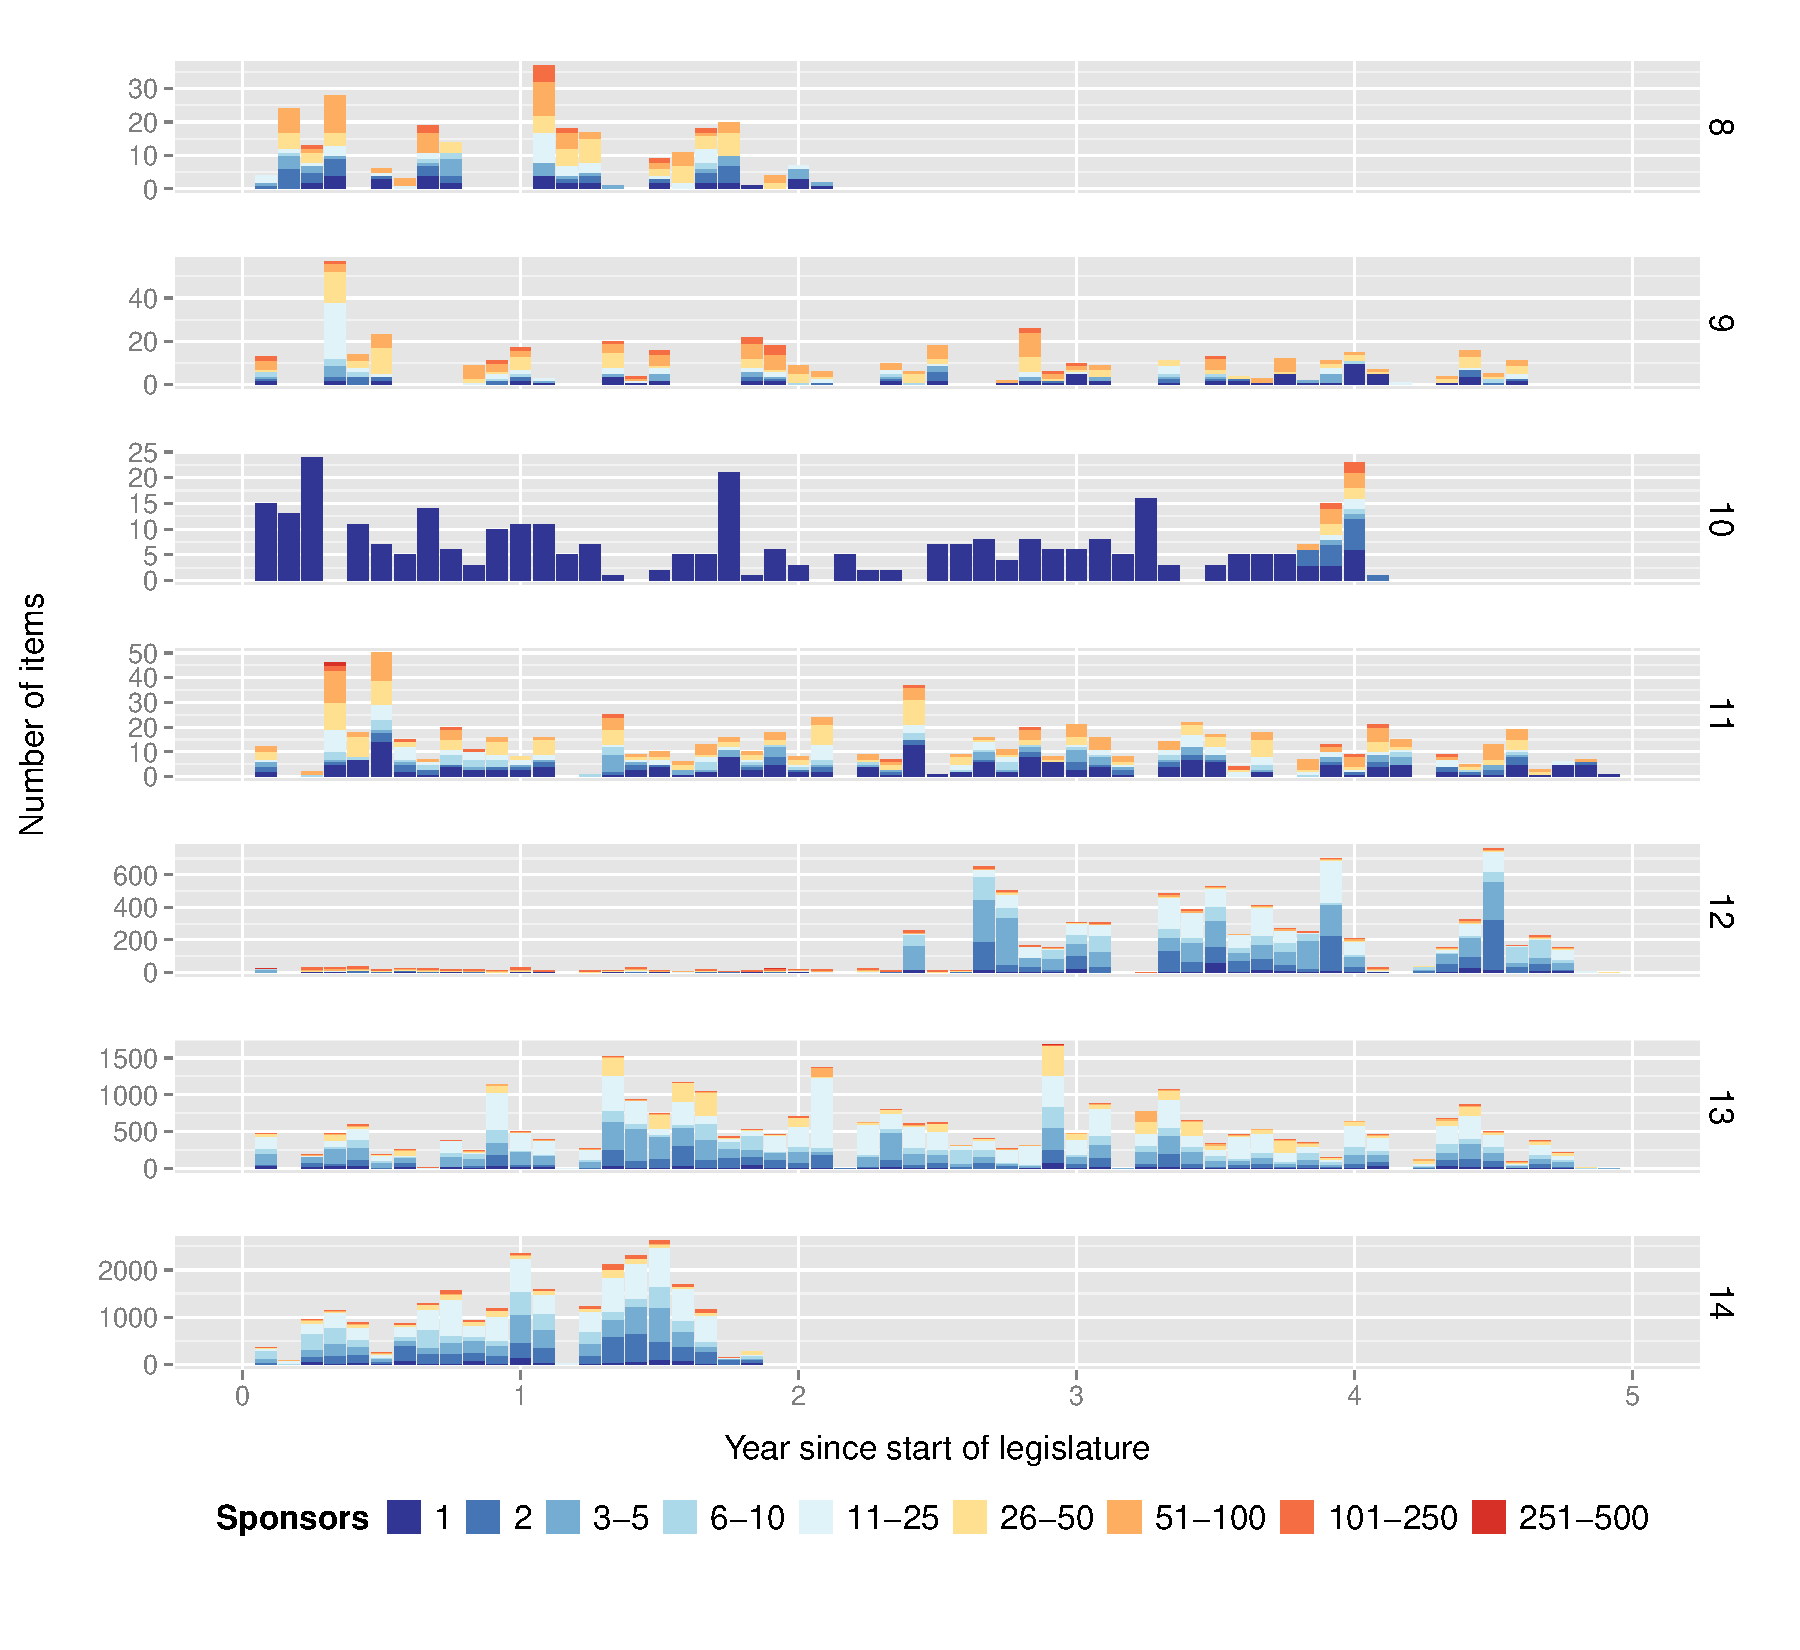
\includegraphics[width=\textwidth]{figures/counts/full_an.pdf}
    \sublegend{National Assembly}%
    \label{fig:counts_an}
  \end{subfigure}

  \begin{subfigure}[t]{.8\textwidth}
    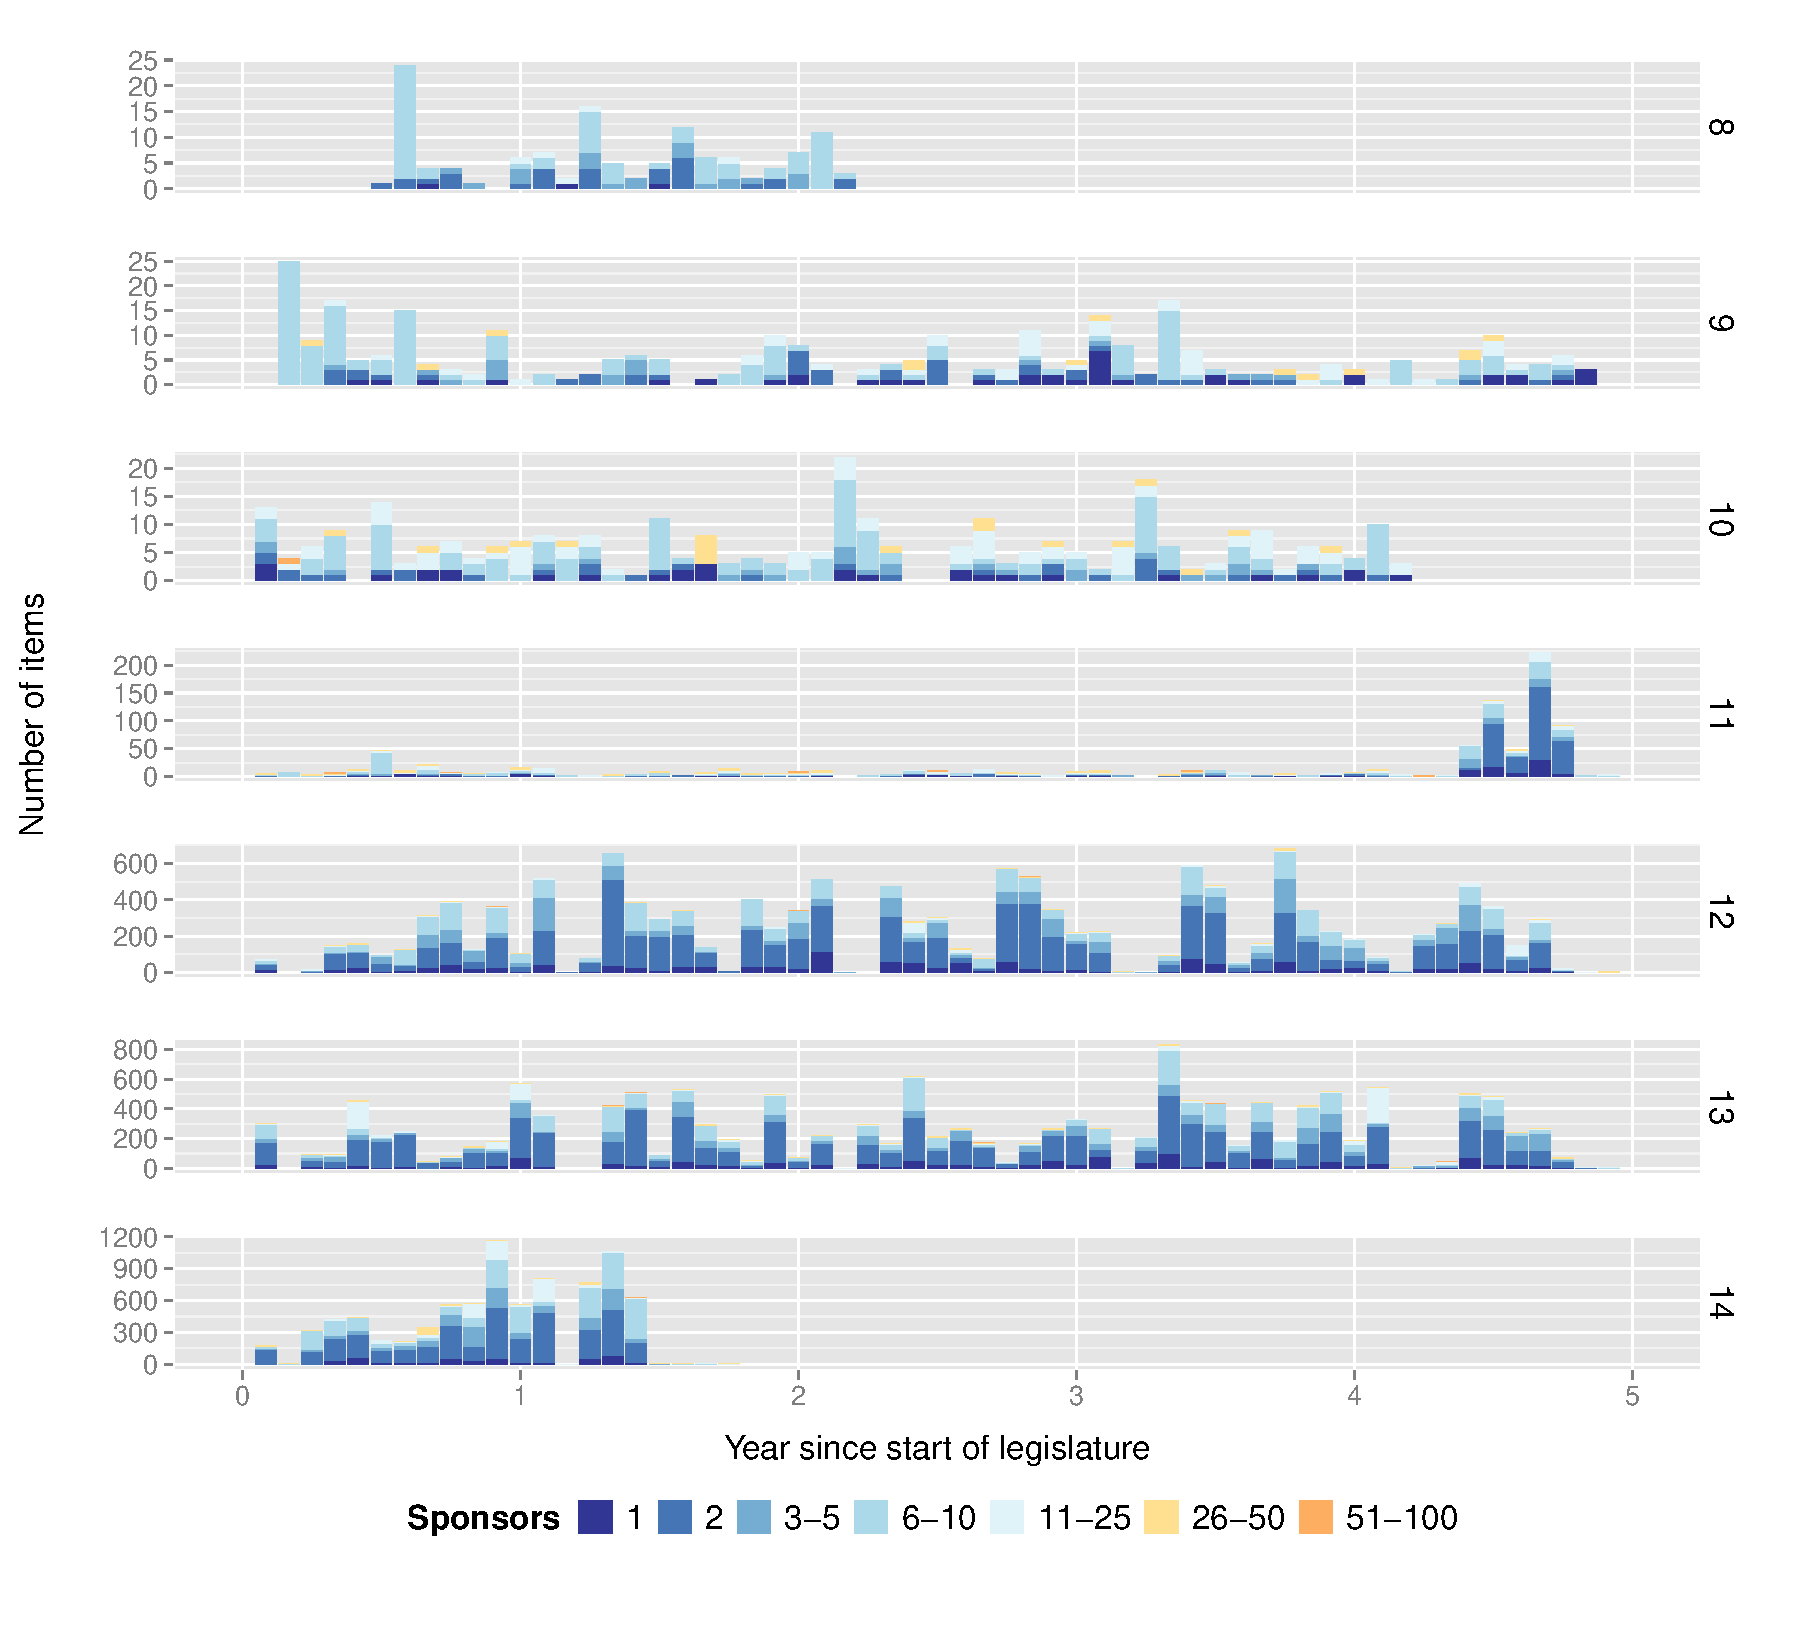
\includegraphics[width=\textwidth]{figures/counts/full_se.pdf}
    \sublegend{Senate}%
    \label{fig:counts_se}
  \end{subfigure}

  \legend{Time distributions of amendments and bills, colored by sponsorships.}%
  \label{fig:counts}
\end{figure}

\clearpage

% TBL. 1

\begin{table}[htbp]
  \centering

  \begin{subtable}[t]{.8\textwidth}
    % latex table generated in R 3.1.0 by xtable 1.7-3 package
% Fri May  9 00:31:21 2014
\begin{tabular}{lrrrrr}
  \hline
Legislature & $\Sigma$~items & $\Sigma$~bills & $\Sigma$~amdts & $\Sigma$~groups & $\Sigma$~sponsors \\ 
  \hline
1986-1988 (8) & 222 & 222 &   0 &   4 & 368 \\ 
  1988-1993 (9) & 388 & 388 &   0 &   4 & 355 \\ 
  1993-1997 (10) &  34 &  34 &   0 &   3 & 378 \\ 
  1997-2002 (11) & 542 & 542 &   0 &   5 & 619 \\ 
  2002-2007 (12) & 7838 & 818 & 7020 &   4 & 677 \\ 
  2007-2012 (13) & 28839 & 1258 & 27581 &   4 & 673 \\ 
  2012-- (14) & 24111 & 550 & 23561 &   6 & 613 \\ 
   \hline
\end{tabular}

    \sublegend{National Assembly}%
    \label{tbl:counts_an}
  \end{subtable}

  \begin{subtable}[t]{.8\textwidth}
    % latex table generated in R 3.1.0 by xtable 1.7-3 package
% Fri May  9 00:31:29 2014
\begin{tabular}{lrrrrr}
  \hline
Legislature & $\Sigma$~items & $\Sigma$~bills & $\Sigma$~amdts & $\Sigma$~groups & $\Sigma$~sponsors \\ 
  \hline
1986-1988 (8) & 128 & 128 &   0 &   5 & 257 \\ 
  1988-1993 (9) & 307 & 307 &   0 &   5 & 387 \\ 
  1993-1997 (10) & 315 & 315 &   0 &   5 & 402 \\ 
  1997-2002 (11) & 953 & 411 & 542 &   5 & 451 \\ 
  2002-2007 (12) & 13687 & 287 & 13400 &   5 & 420 \\ 
  2007-2012 (13) & 14601 & 542 & 14059 &   6 & 524 \\ 
  2012-- (14) & 8363 & 204 & 8159 &   6 & 454 \\ 
   \hline
\end{tabular}

    \sublegend{Senate}%
    \label{tbl:counts_se}
  \end{subtable}

  \legend{Total counts of amendments, bills, unique party groups and MP sponsors over legislatures 8--14 (1986-2014).}%
  \label{tbl:counts}
\end{table}

\clearpage

% FIG. 2

\begin{figure}[htbp]
  \centering

  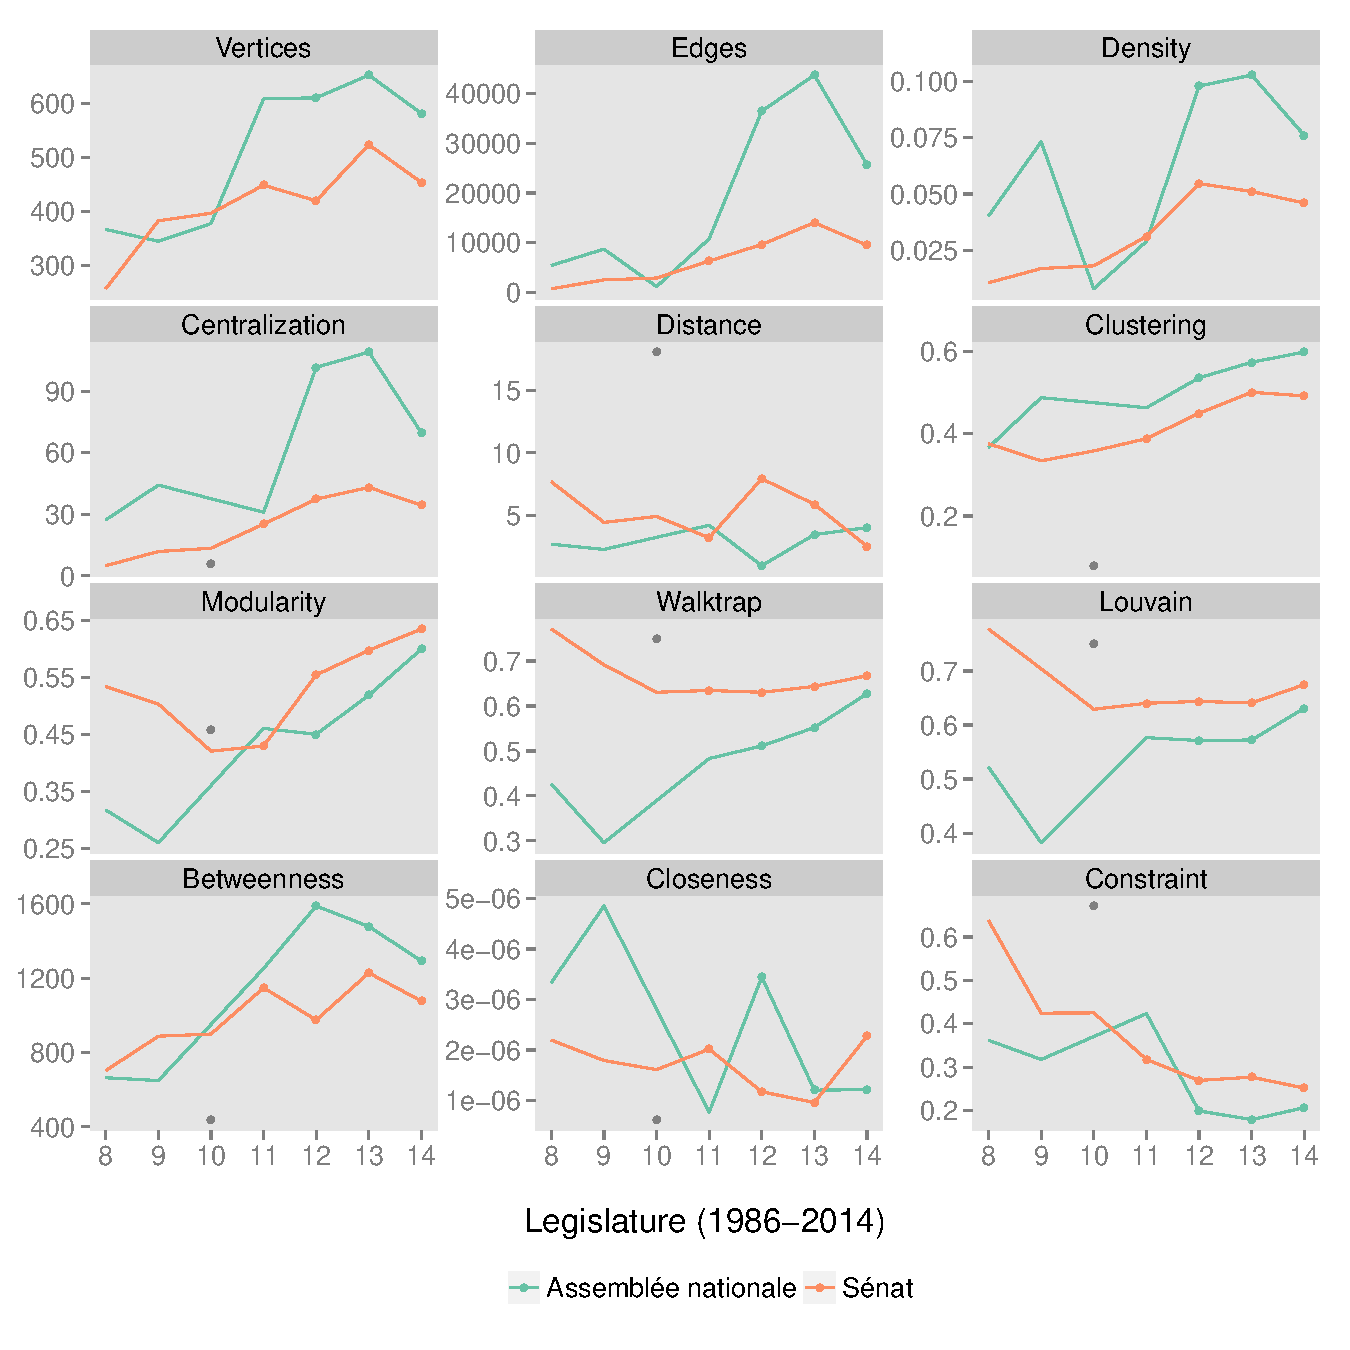
\includegraphics[width=\textwidth]{figures/measures/full.pdf}

  \legend{Graph-level properties of the cosponsorship networks. Estimates that include amendments in addition to bills are shown with dots. Legislature 10 of the National Assembly is shown as a grey dot due to very sparse network data.}%
  \label{fig:measures}
\end{figure}

\clearpage

% TBL. 2

\begin{table}[htbp]
  \centering

  \begin{subtable}[t]{.8\textwidth}
    % latex table generated in R 3.1.0 by xtable 1.7-3 package
% Sat May 10 20:48:56 2014
\begin{tabular}{lrrr}
  \hline
Legislature & Modularity & $\max{M}$ & $M / \max{M}$ \\ 
  \hline
1986-1988 (8) & 0.32 & 0.52 & 0.61 \\ 
  1988-1993 (9) & 0.26 & 0.38 & 0.68 \\ 
  1993-1997 (10) & 0.46 & 0.75 & 0.61 \\ 
  1997-2002 (11) & 0.46 & 0.58 & 0.80 \\ 
  2002-2007 (12) & 0.45 & 0.57 & 0.79 \\ 
  2007-2012 (13) & 0.52 & 0.57 & 0.91 \\ 
  2012-- (14) & 0.60 & 0.63 & 0.95 \\ 
   \hline
\end{tabular}

    \sublegend{National Assembly}%
    \label{tbl:modularity_an}
  \end{subtable}

  \begin{subtable}[t]{.8\textwidth}
    % latex table generated in R 3.1.0 by xtable 1.7-3 package
% Sat May 10 20:49:00 2014
\begin{tabular}{lrrr}
  \hline
Legislature & Modularity & $\max{M}$ & $M / \max{M}$ \\ 
  \hline
1986-1988 (8) & 0.53 & 0.78 & 0.69 \\ 
  1988-1993 (9) & 0.50 & 0.70 & 0.71 \\ 
  1993-1997 (10) & 0.42 & 0.63 & 0.67 \\ 
  1997-2002 (11) & 0.43 & 0.64 & 0.67 \\ 
  2002-2007 (12) & 0.55 & 0.64 & 0.86 \\ 
  2007-2012 (13) & 0.60 & 0.64 & 0.93 \\ 
  2012-- (14) & 0.63 & 0.67 & 0.94 \\ 
   \hline
\end{tabular}

    \sublegend{Senate}%
    \label{tbl:modularity_se}
  \end{subtable}

  \legend{Network party-based modularity, compared to its algorithmic maximization, $\max M$, and to their ratio.}% `Delta' columns indicate how many communities were identified by the maximization algorithms past the actual number of party groups in the legislature.}%
    %
    % Further diagnostics for each method are included in the replication material, along with with sensitivity tests for the weighting parameter \citep{OpsahlAgneessens2010-SN}.}
    %
  \label{tbl:modularity}
\end{table}

\clearpage

% FIG. 3

\begin{figure}[htbp]
  \centering

  \begin{subfigure}[t]{.8\textwidth}
    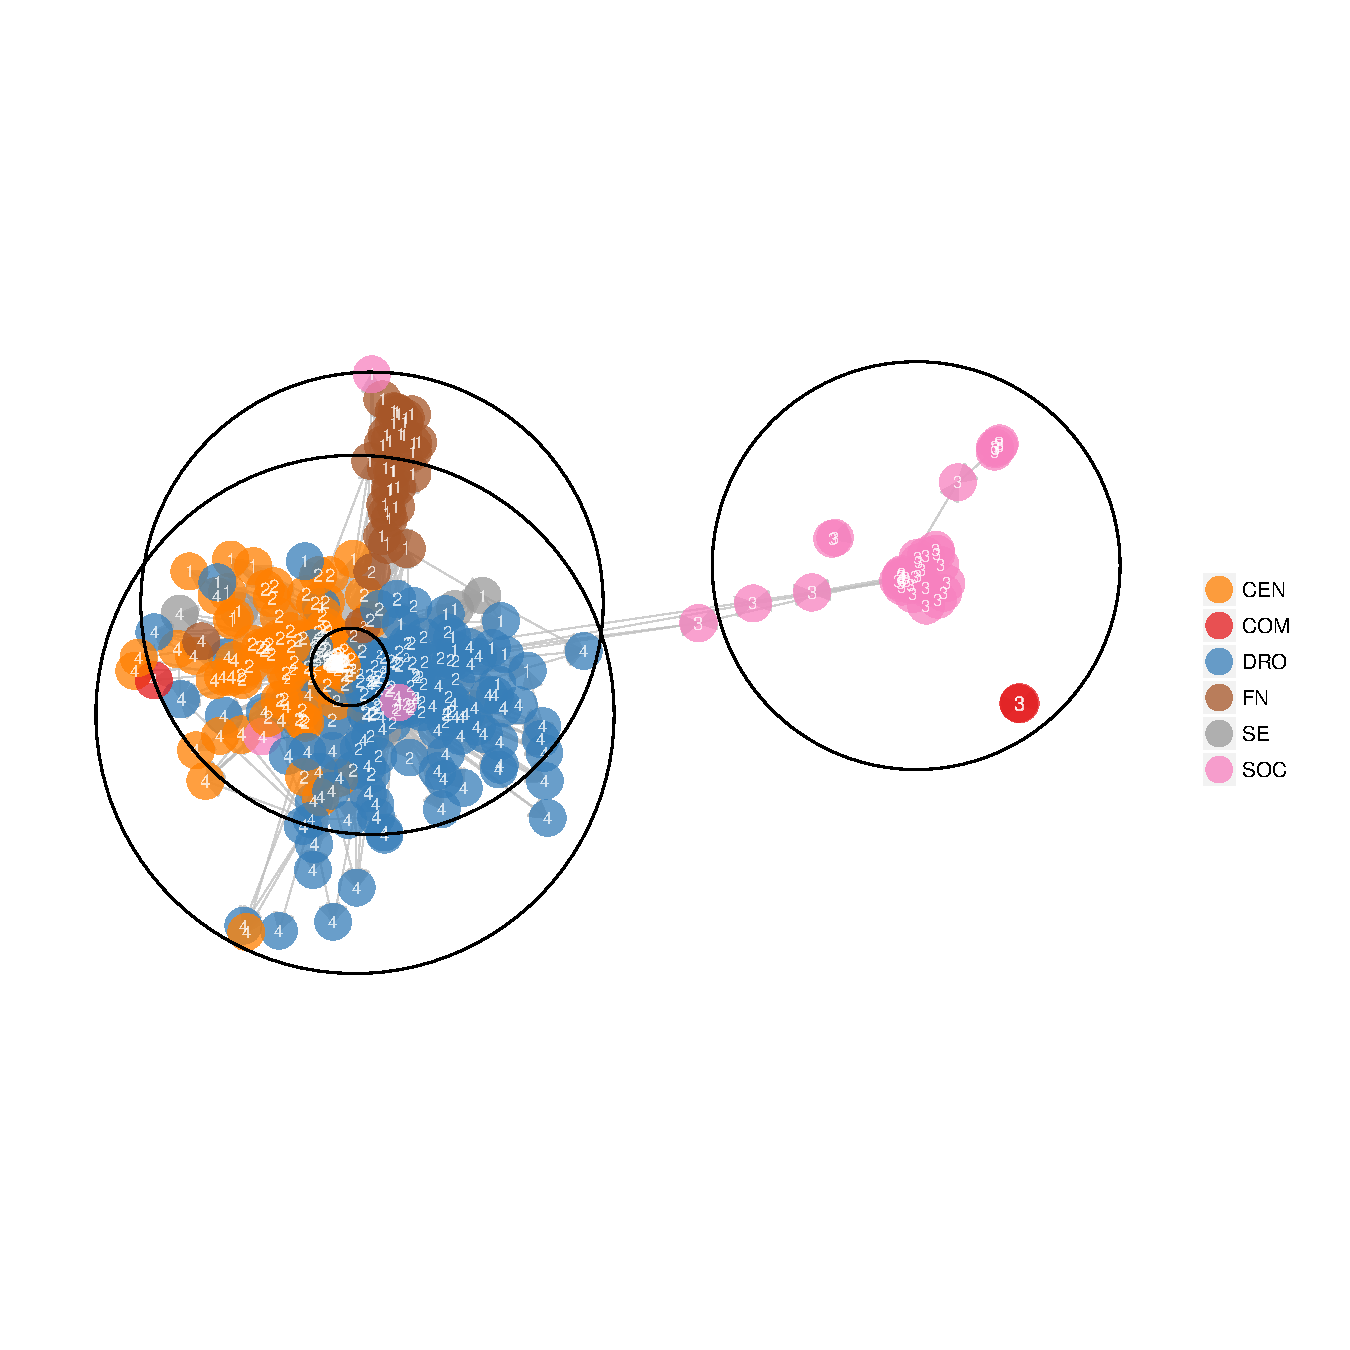
\includegraphics[width=\textwidth]{figures/an8_ergmm.pdf}
    \sublegend{Latent space positions}%
    \label{fig:an8_ergmm}
  \end{subfigure}

  \begin{subfigure}[t]{.8\textwidth}
    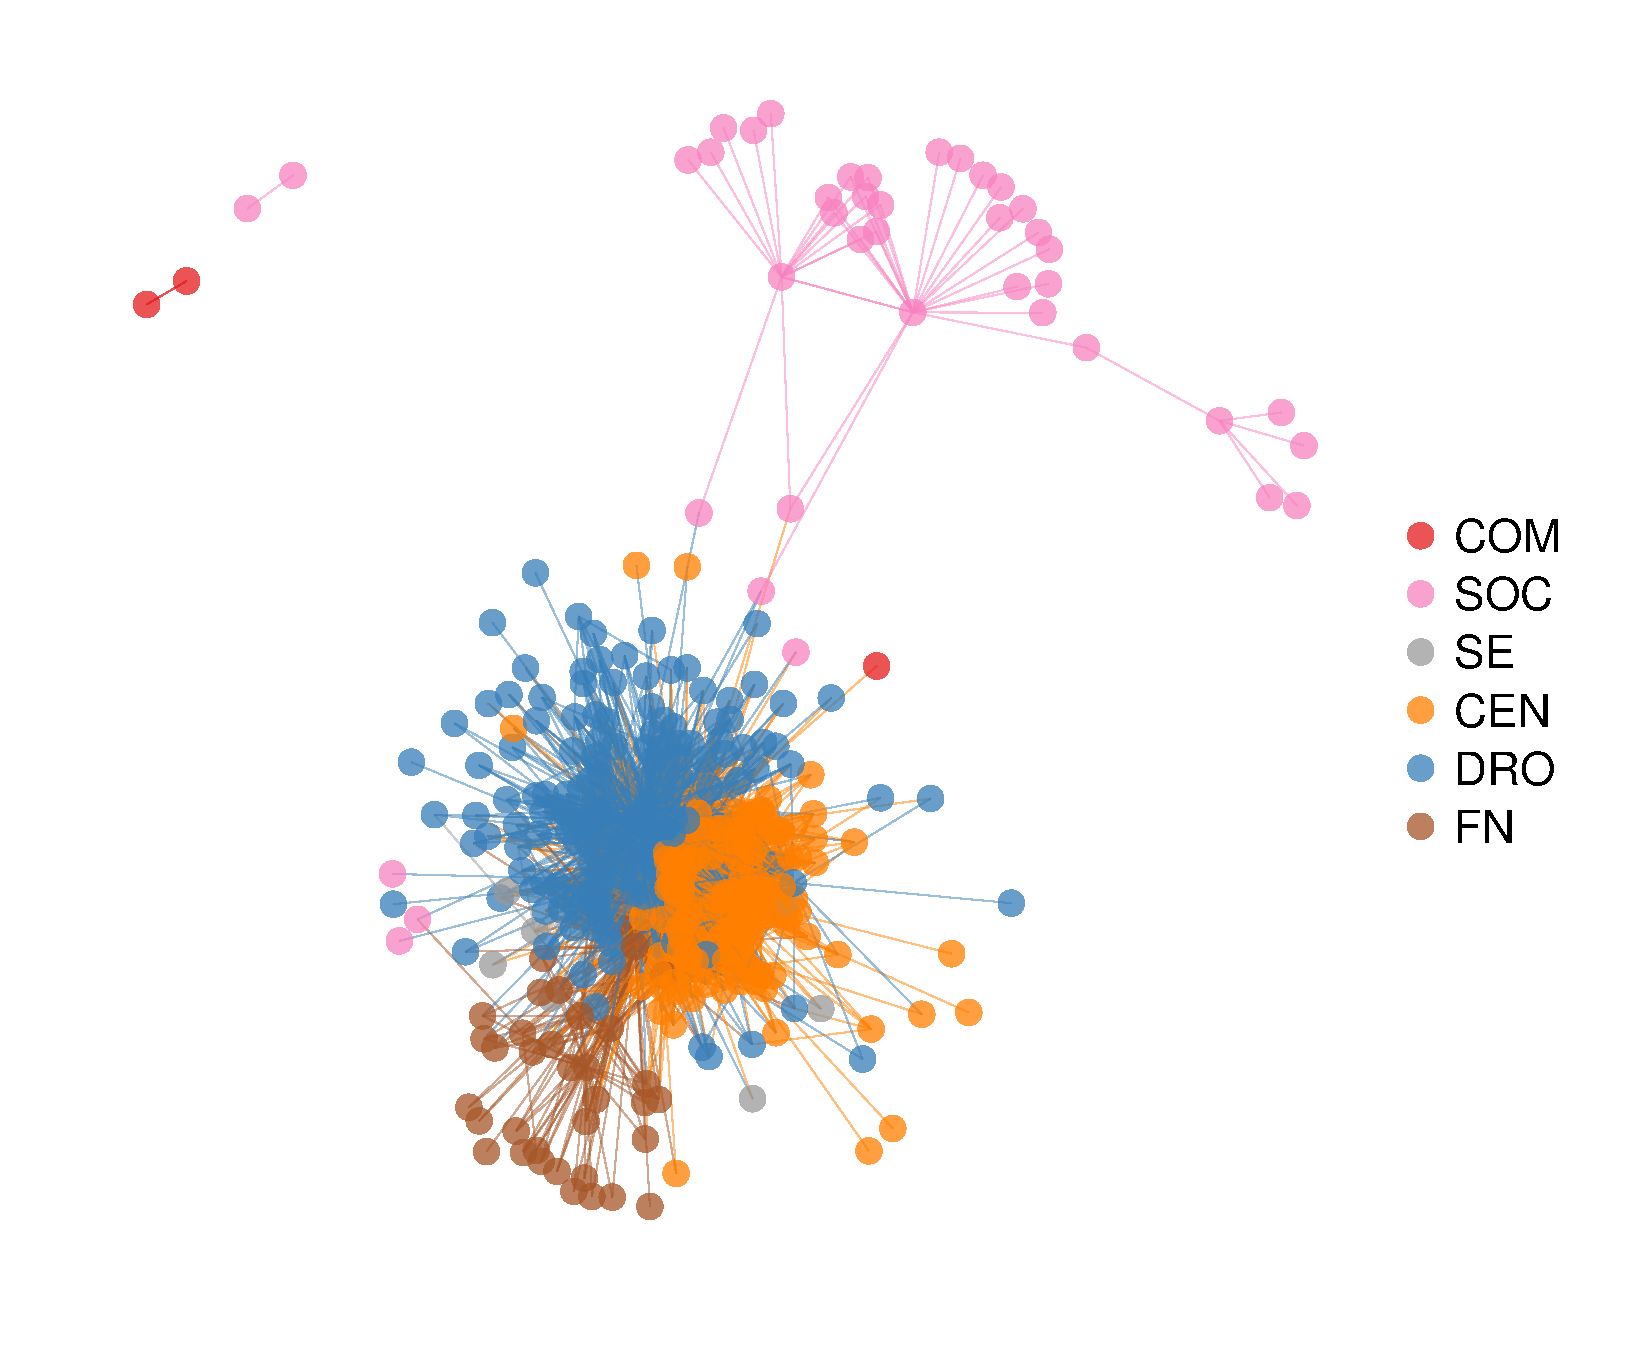
\includegraphics[width=\textwidth]{figures/an8.pdf}
    \sublegend{Force-directed graph}%
    \label{fig:an8}
  \end{subfigure}

  \legend{Network representations of the National Assembly under legislature~8 (1986--1988). Colors correspond to actual party colors, and numbers correspond to $K = 4$ latent cluster memberships. Circle positions and diameters are proportional to latent cluster means and variances.}%
  \label{fig:ergmm_an}
\end{figure}

\clearpage

% FIG. 4

\begin{figure}[htbp]
  \centering

  \begin{subfigure}[t]{.8\textwidth}
    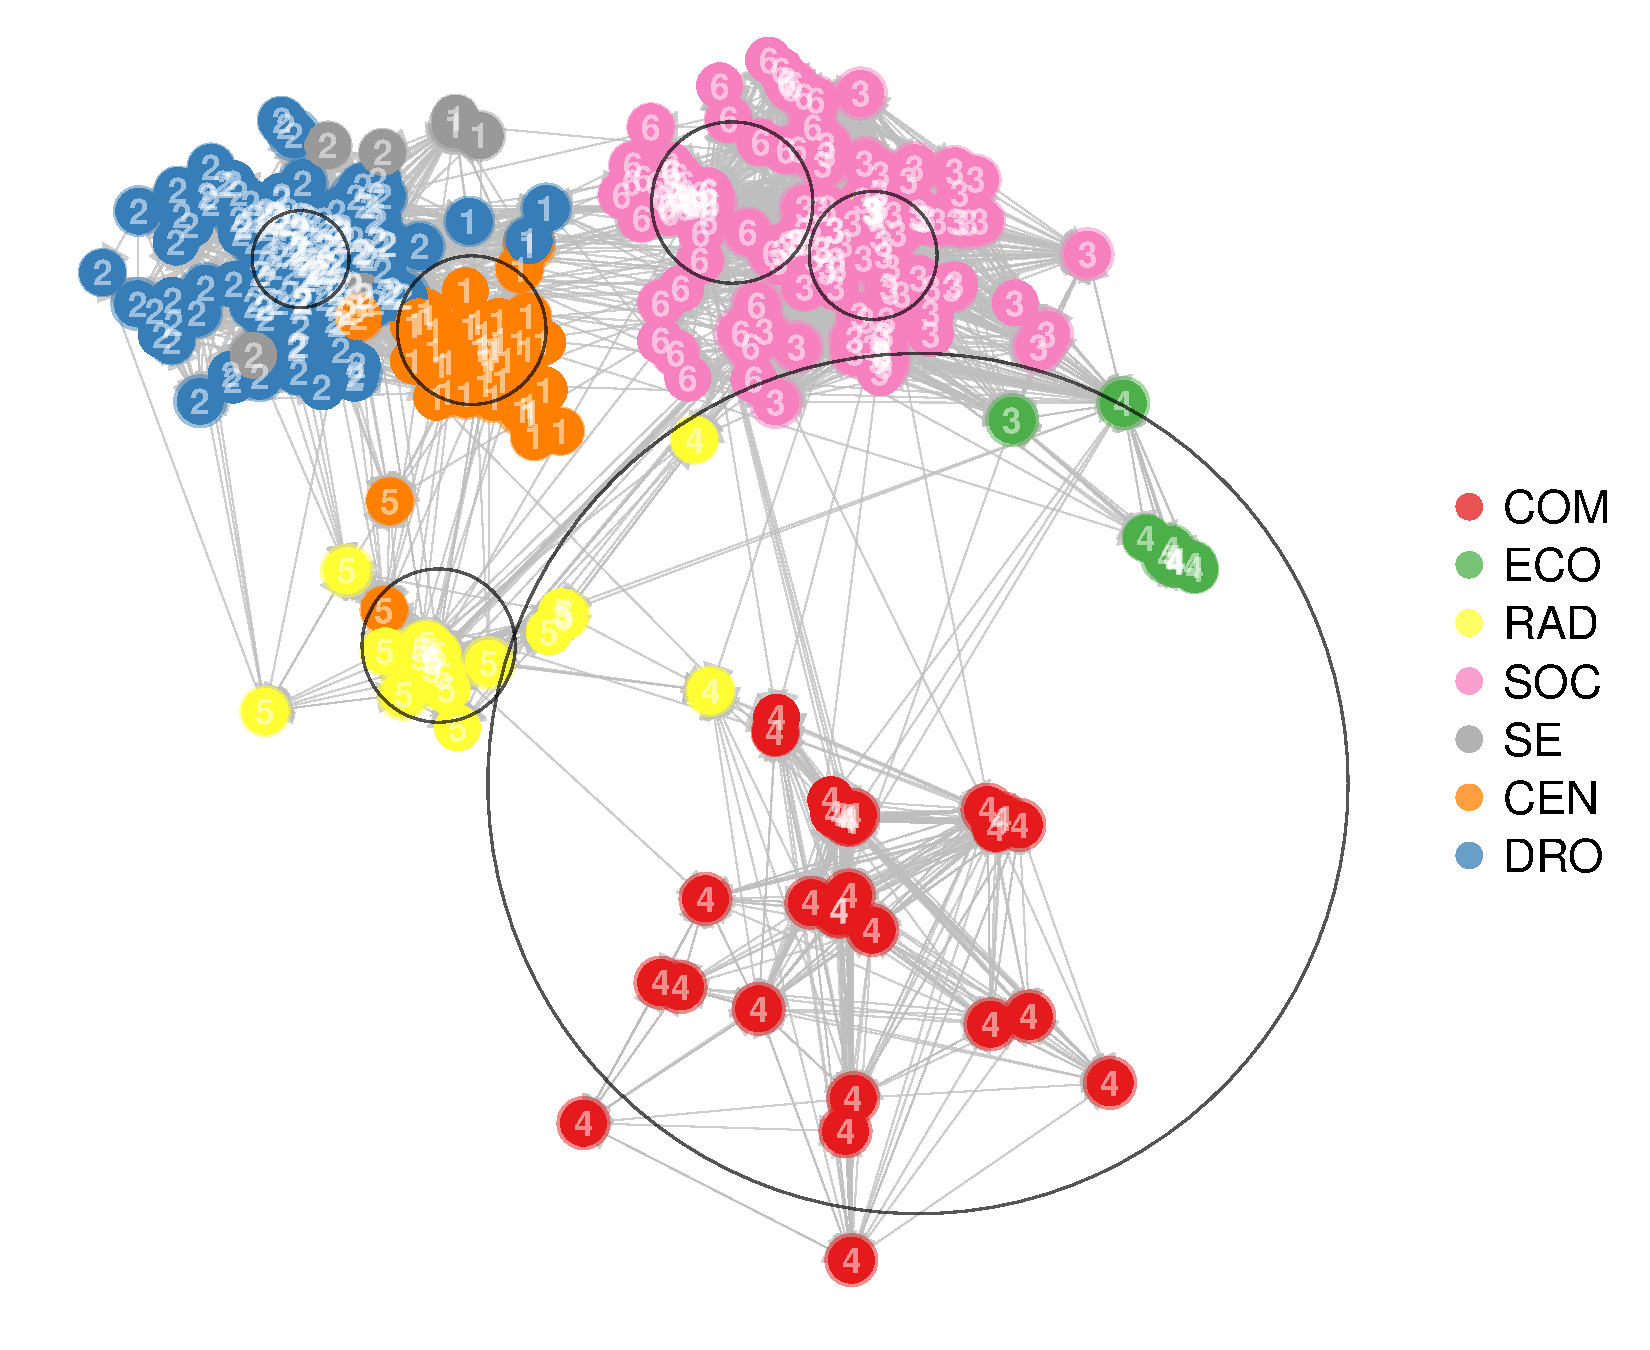
\includegraphics[width=\textwidth]{figures/se14_ergmm.pdf}
    \sublegend{Latent space positions}%
    \label{fig:ergmm_se14}
  \end{subfigure}

  \begin{subfigure}[t]{.8\textwidth}
    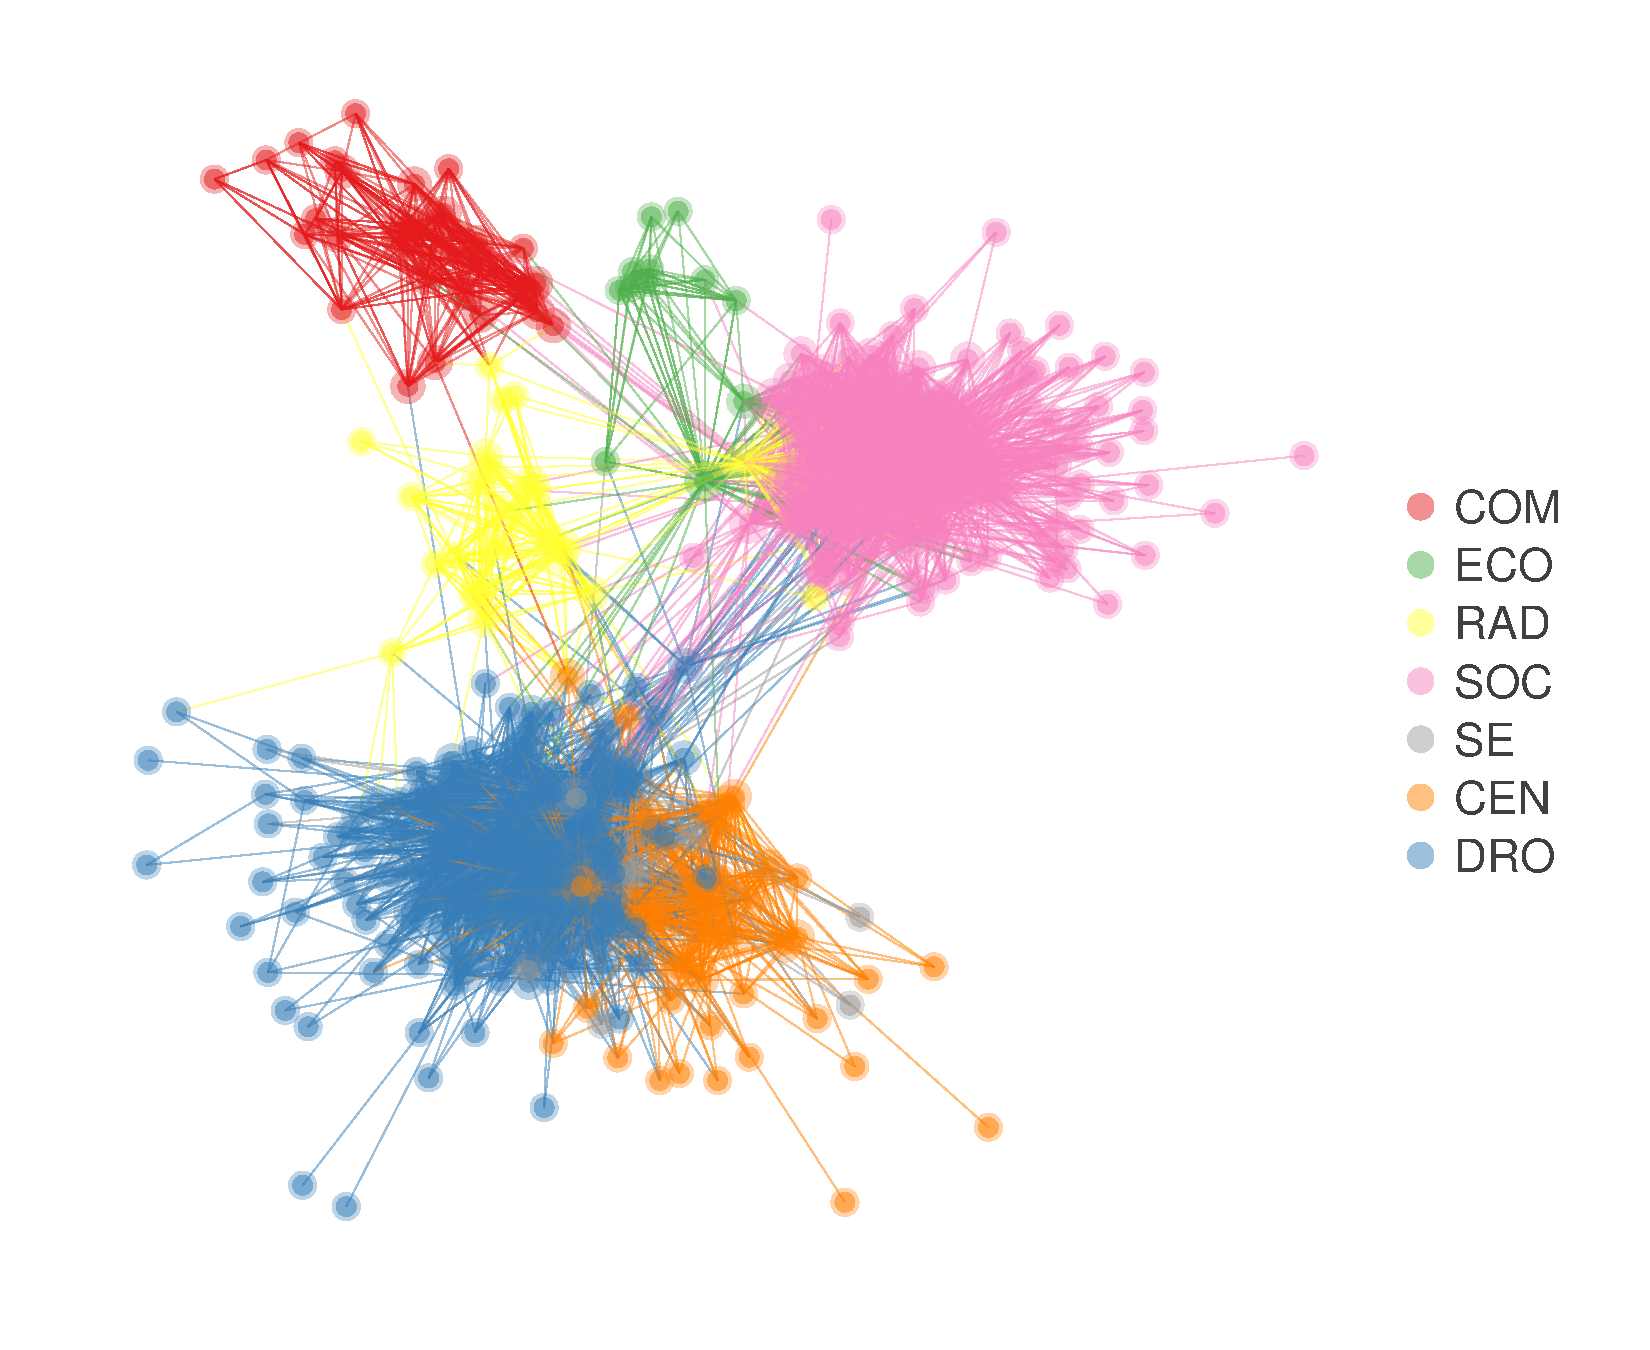
\includegraphics[width=\textwidth]{figures/se14.pdf}
    \sublegend{Force-directed graph}%
    \label{fig:se14}
  \end{subfigure}

  \legend{Network representations of the Senate under legislature~14 (2012--). Colors correspond to actual party colors, and numbers correspond to $K = 4$ latent cluster memberships. Circle positions and diameters are proportional to latent cluster means and variances.}%
  \label{fig:ergmm_se}
\end{figure}

\clearpage

% FIG. 5

\begin{figure}[htbp]
  \centering

  \includegraphics[width=\textwidth]{figures/fm.pdf}

  \legend{Fowlkes-Mallows indices for the latent cluster random effects models.}%
  \label{fig:fm}
\end{figure}

\clearpage

% FIG. 6

\begin{figure}[htbp]
  \centering

  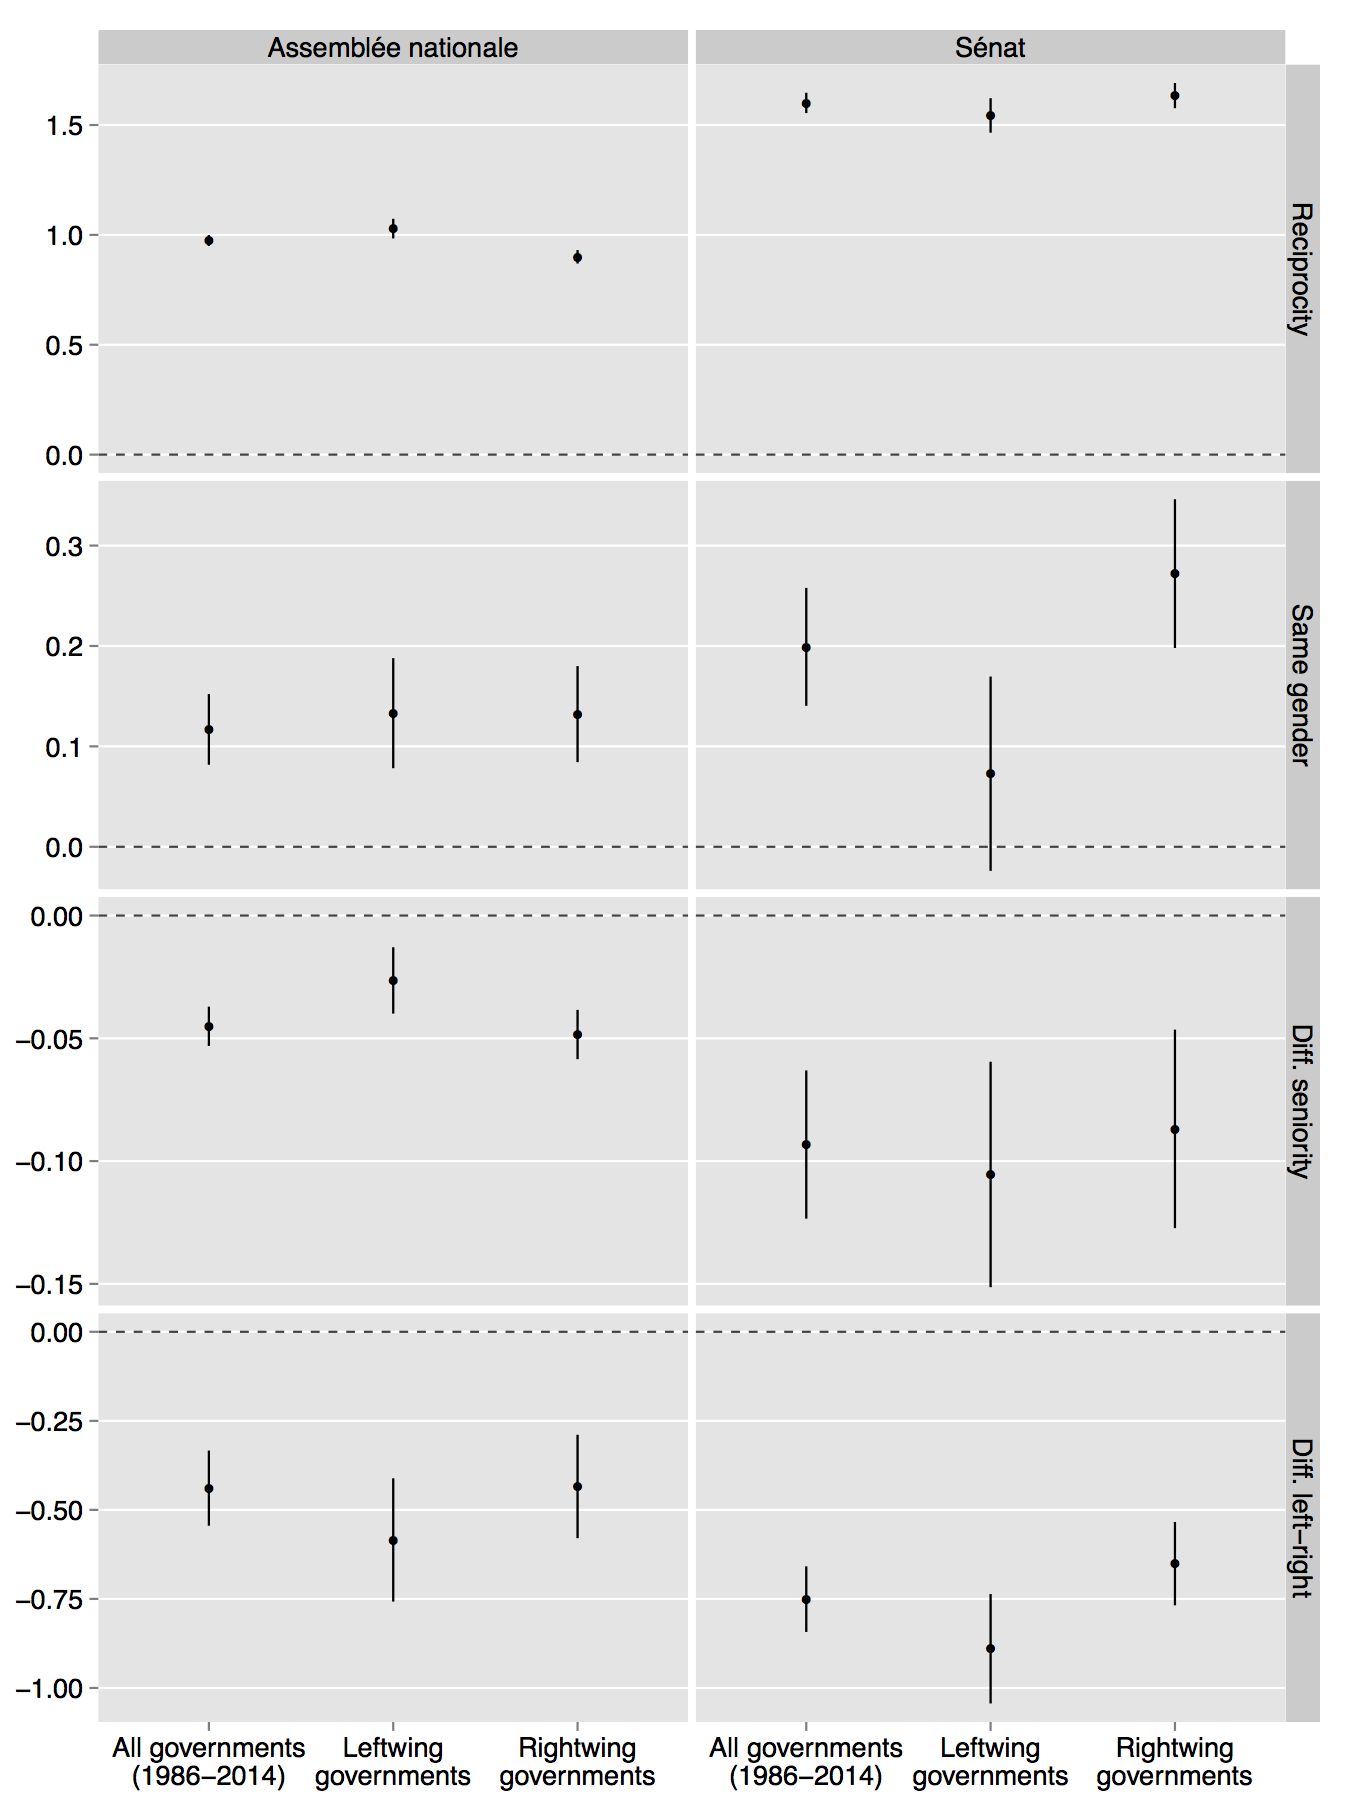
\includegraphics[width=\textwidth]{figures/ergm_cov.pdf}

  \legend{ERGM coefficients for all legislatures. Full model coefficients are net of the within-party homophily effects reported in Figure~\ref{fig:ergm_diff}. Estimates are not shown when their standard error exceeds two thirds of their magnitude.}%
  \label{fig:ergm_beta}
\end{figure}

\clearpage

% FIG. 7

\begin{figure}[htbp]
  \centering

  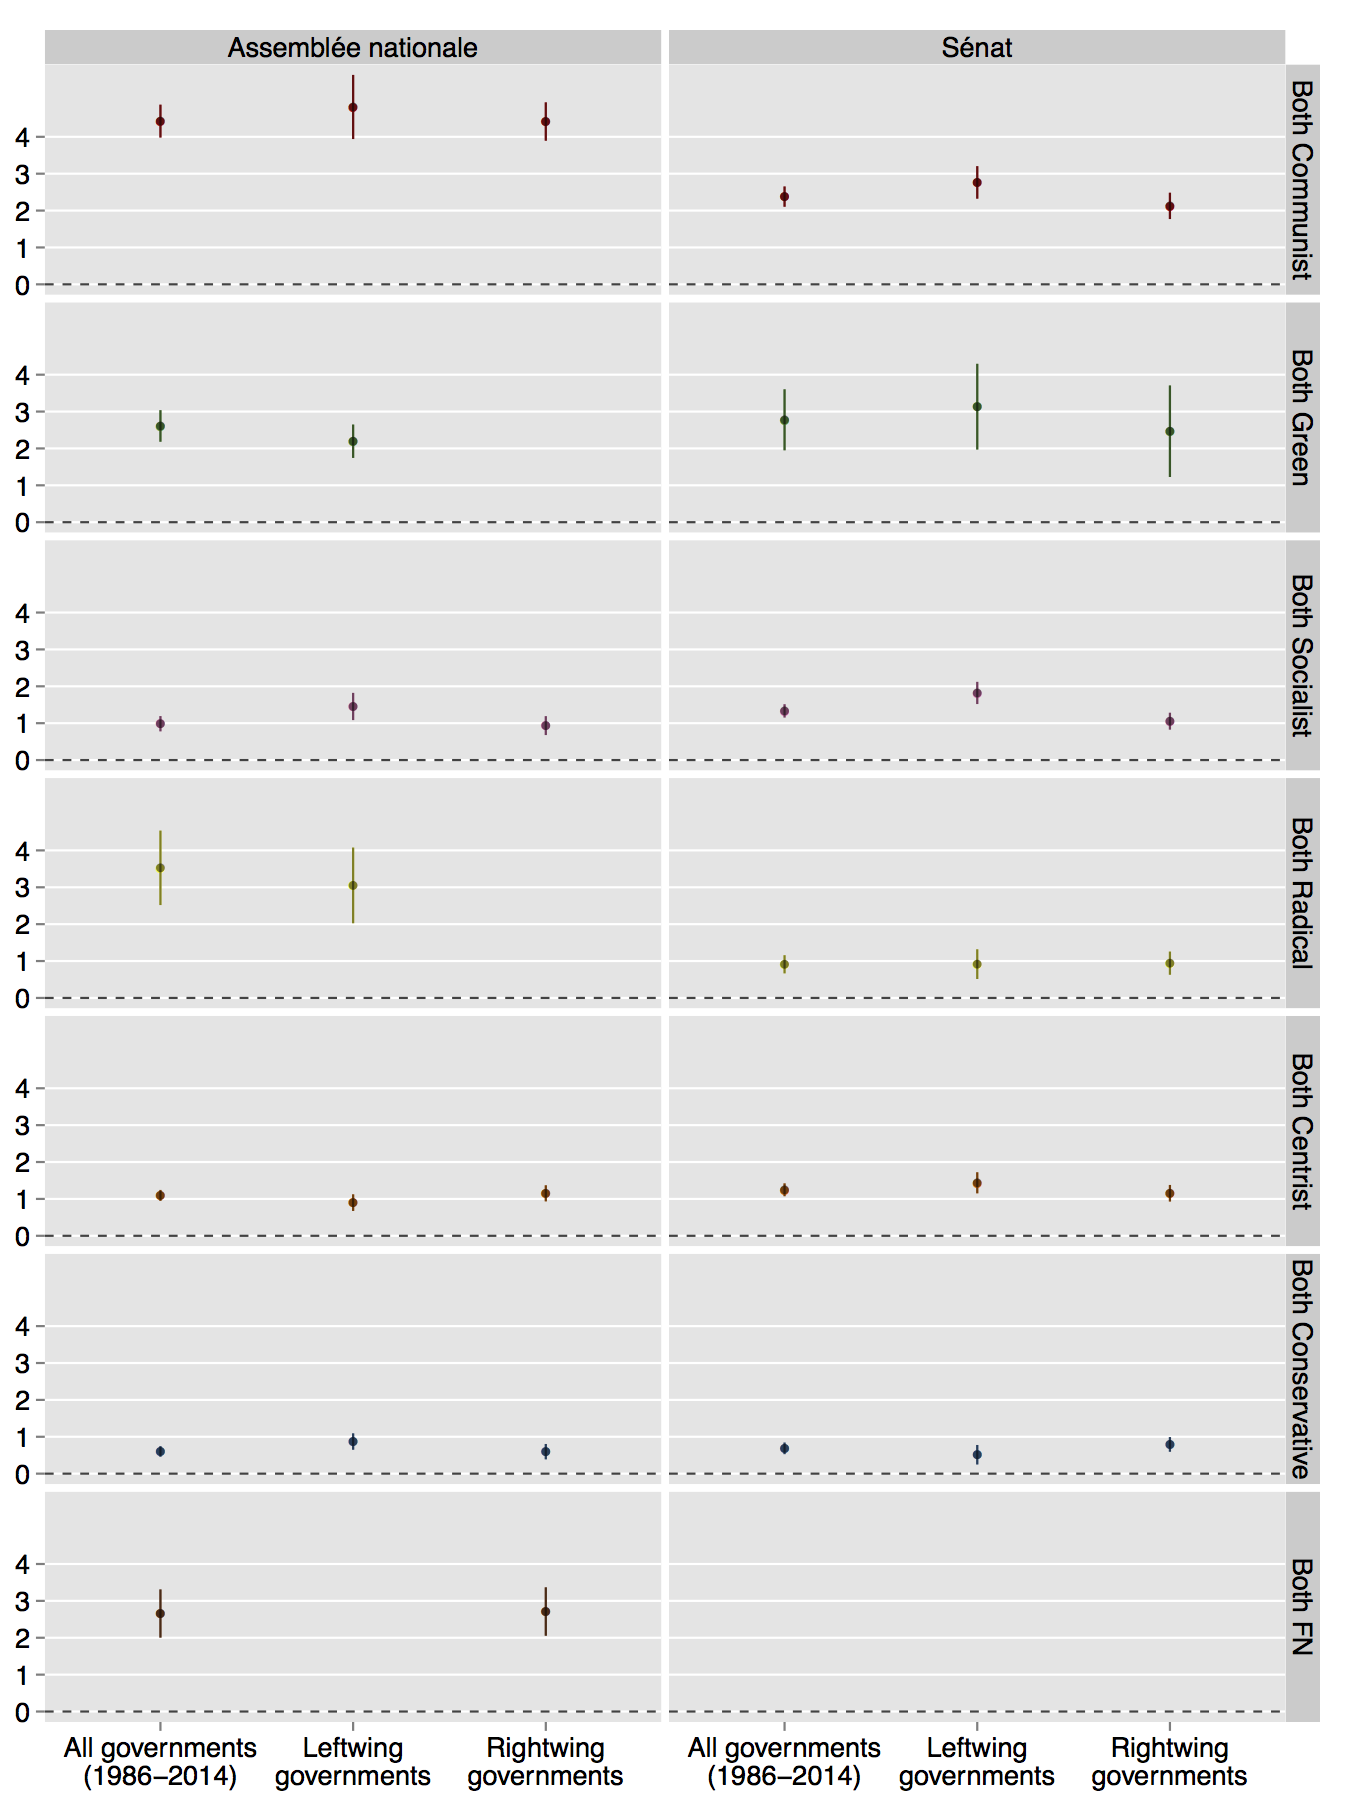
\includegraphics[width=\textwidth]{figures/ergm_diff.pdf}

  \legend{ERGM within-party homophily coefficients for all legislatures. All coefficients are net of the covariate effects reported in Figure~\ref{fig:ergm_beta} and are not shown when their standard error exceeds two thirds of their magnitude. Only one point estimate was initially measured for Radicals in the National Assembly.}%
  \label{fig:ergm_diff}
\end{figure}

\clearpage

% TBL. 4

\input{tables/ergm_an}

\clearpage

% TBL. 5

\input{tables/ergm_se}

%   \centering
%   \footnotesize{Typeset on \today~with \TeX{} and \href{http://yihui.name/knitr/}{\texttt{knitr}} in \href{http://rstudio.org/}{RStudio}, \\ using the \emph{Political Analysis} style by Jonathan N. Katz.}

\end{document}
